% Hinweis: Um das finale Dokument zu erstellen, als weitere Option "final" angeben
% Dies versteckt u.a. TODO-Elemente
\documentclass[12pt,final]{report}
%für finale Version
%documentclass[12pt,final]{report}
\usepackage{style}
\usepackage{dhbwTitlepage} % Eigene Titelseite verwenden


% "Metadaten"
\title{\Large{Evaluierung von Tools zum Auffinden von Undefined Behavior}}
\project{T3000}
\author{Christoph Böhringer}
\supervisor{Dipl.-Inform. (FH) Thomas Weller}
\studentNumber{3275565}
\class{TINF18-IN}
\company{Mitutoyo CTL Germany GmbH}
\date{21.06.2021}

% Initialisierungen für Abkürzungsverzeichnis
\makenoidxglossaries
\loadglsentries{Acronyms.tex}

\addbibresource{literature.bib}

\begin{document}

\pagenumbering{Roman}

\maketitle
\chapter*{Erklärung}
\label{ch:erklaerung}

Ich versichere hiermit, dass ich meine 
\makeatletter
\@project
\makeatother
\ mit dem Thema 
\makeatletter
\glqq{}\@title\grqq{}
\makeatother
\ selbstständig verfasst und keine anderen als die angegebenen Quellen und Hilfsmittel benutzt habe.

Ich versichere zudem, dass die eingereichte elektronische Fassung mit der gedruckten Fassung übereinstimmt.

Falls gleichwertige Entscheidungen getroffen werden mussten, wurden diese von mir
entschieden, außer es ist anders angegeben.

\vspace{2.0cm}
\underline{\hspace{12cm}}\\
Ort \hspace{3cm} Datum \hspace{2cm} 
\makeatletter
\@author
\makeatother
\chapter*{Abstract}
\label{ch:abstract}
\addcontentsline{toc}{chapter}{\nameref{ch:abstract}}
In einem Softwareprodukt trat bei der Umstellung von 32 Bit auf 64 Bit ein Fehler auf,
dessen Ursache sich vermutlich auf Undefined Behavior von C++ zurückführen lässt. Diese Arbeit soll den Nachweis erbringen oder widerlegen,
dass Undefined Behavior die Ursache für den Fehler war. Optional kann eine mögliche Erklärung gesucht werden,
warum der betroffene Code in der 32 Bit Version keinen Fehler verursacht hat.

Das betroffene Projekt wurde vor der Umstellung mehrere Jahre lang nicht verändert. Es muss daher davon ausgegangen werden,
dass sich ähnliche Fehler damals auch an anderen Stellen eingeschlichen haben, jedoch noch nicht  bemerkt wurden.
Die Arbeit soll untersuchen, ob weitere Fehler vom Typ Undefined Behavior in diesem Projekt vorliegen.

Um Fehler dieser Art auch in anderen Projekten auszuschließen, sollen Tools gesucht und evaluiert werden,
mit denen die Fehler automatisiert gefunden und berichtet werden können. Falls kein passendes Tool existiert, soll aufgezeigt werden,
mit welchem manuellen Vorgehen solche Stellen erkannt werden können.

Die Tools sollen möglichst mit den bestehenden Entwicklungsumgebungen verwendet werden können und idealerweise alle Arten von
Undefined Behavior erkennen.

Hinweis: Da in der Arbeit Source Code der Mitutoyo CTL Germany GmbH offengelegt wird, ist die Arbeit unter Verschluss zu halten.

\tableofcontents
\listoffigures
\listoftables
\printnoidxglossary[type=\acronymtype, title={Abkürzungen}, nogroupskip]
\printnoidxglossary[type=main]
%%%%%%%%%%%%% Inhalt %%%%%%%%%%%%%

\clearpage
\pagenumbering{arabic}

\chapter{Einleitung}
\label{ch:Einleitung}

In einem Softwareprodukt trat bei der Umstellung von 32 Bit auf 64 Bit ein Fehler auf,
dessen Ursache sich vermutlich auf Undefined Behavior von C++ zurückführen lässt. Diese Arbeit soll den Nachweis erbringen oder widerlegen,
dass Undefined Behavior die Ursache für den Fehler war. Optional kann eine mögliche Erklärung gesucht werden,
warum der betroffene Code in der 32 Bit Version keinen Fehler verursacht hat.

Das betroffene Projekt wurde vor der Umstellung mehrere Jahre lang nicht verändert. Es muss daher davon ausgegangen werden,
dass sich ähnliche Fehler damals auch an anderen Stellen eingeschlichen haben, jedoch noch nicht  bemerkt wurden.

Um Fehler dieser Art auch in anderen Projekten auszuschließen, sollen Tools gesucht und evaluiert werden,
mit denen die Fehler automatisiert gefunden und berichtet werden können. Falls kein passendes Tool existiert, soll aufgezeigt werden,
mit welchem manuellen Vorgehen solche Stellen erkannt werden können.

Die Tools sollen möglichst mit den bestehenden Entwicklungsumgebungen verwendet werden können und idealerweise alle Arten von
Undefined Behavior erkennen.

\chapter{Small Talk}
\label{ch:smalltalk}

\section{Was ist Small Talk?}
\label{sec:smalltalk_was}

Als Small Talk (engl. \textit{small} \glqq{}unbedeutend, klein\grqq{} und \textit{to talk} \glqq{}sich unterhalten\grqq{}) wird ein spontanes, zufällig entstandenes, lockeres Gespräch
bezeichnet. Die häufigsten Themen beziehen sich dabei meist auf das Privatleben der Involvierten, oder auf das Geschehen um das Gespräch. Der Ton des Gesprächs ist informell.\cite{misc:wikipedia_smalltalk} \newline
Im Alltag kann es in verschiedenen Situationen zu einem Small Talk kommen:
\begin{itemize}
    \item Auf dem Weg zur Arbeit
    \item In der Mittagspause
    \item Beim Einkaufen
    \item Beim Spazierengehen
    \item An der Supermarktkasse
    \item In öffentlichen Verkehrsmitteln
    \item Auf einer Party
    \item \dots
\end{itemize}

Small Talk kann in verschiedenen Situationen, beispielsweise in einem Bewerbungsgespräch, als \glqq{}Eisbrecher\grqq{} verwendet werden. Das Führen von Small Talk hilft dabei Interesse am
Gegenüber zu zeigen. In einem beruflichen Umfeld können somit Beziehungen zu Kollegen/-innen geknüpft werden. \newline
Die Auswahl der Gesprächsthemen orientiert sich dabei daran, wie gut man das Gegenüber bereits kennt. Handelt es sich um eine/-n Freund/-in, so kann der Small Talk auch übersprungen werden
und das Gespräch kann mit einem bevorzugten Thema begonnen werden. \cite{misc:wikipedia_smalltalk}

\section{Small Talk führen}
\label{sec:smalltalk_führen}

Typische Fragen im Small Talk, wie
\begin{itemize}
    \item Wie findest du das Wetter?
    \item Wie geht es dir/deiner Familie?
\end{itemize}
können als Gesprächseinstieg dienen, sind aber nicht weiterführend und können somit die Konversation zum Stehen bringen.  \newline
Offene Fragen, also Fragen welche nicht mit \glqq{}Ja\grqq{} oder \glqq{}Nein\grqq{} beantwortet werden können, erfordern eine detailliertere Antwort vom Gegenüber und fördern somit den
Gesprächsfluss. Beispiele für Anfänge einer offenen Frage sind \glqq{}Warum\grqq{} oder \glqq{}Was\grqq{}.

Gemeinsamkeiten, wie der Ort des Gespräches, stellen eine gute Grundlage für Themen dar. Durch diese wird eine vertraute Atmosphäre geschaffen. \cite[S.~104]{Birgelen:Ich-und-der-Kunde} \newline
Während des Small Talks bietet es sich an, öfters das Thema zu wechseln. Small Talk ist ein unbeschwertes Gespräch und wird durch Themenwechsel abwechslungsreich, leicht und locker. \cite[S.~108]{Birgelen:Ich-und-der-Kunde}

Neben der allgemeinen Gesprächsführung spielen, für eine gelungene Konversation, auch Mimik, Gestik und Haltung eine Rolle. \newline
Bei der Mimik ist hierbei auf Augenkontakt zu achten, schüchterne Menschen können dabei auch auf den Mund schauen. Des Weiteren haben ein Lächeln und das Vermeiden von Grimassen einen
positiven Einfluss auf das Gespräch. \newline
Das Verwenden der Arme und Hände zur Gestikulation in einem Gespräch machen dieses lebendiger. Eine belebte Körpersprache zeigt Offenheit und Extraversion. Versteckte Handflächen
und verschränkte Arme deuten hingegen auf Verschlossenheit hin. \cite[S.~119]{Birgelen:Ich-und-der-Kunde} \newline
Eine starke und selbstbewusste Haltung zieht Aufmerksamkeit auf den/die Redner/-in. Dies kann auch das Selbstbewusstsein des/der Redners/-in steigern, was schüchternen Menschen bei der
Gesprächsführung helfen kann. Zu einer selbstbewussten Körperhaltung gehören: \cite{misc:rhetorik_selbstbewusstsein}
\begin{itemize}
    \item Fester Stand: beide Beine fest und ungefähr schulterbreit auf dem Boden
    \item Aufrechte Schultern
    \item Gerader Rücken
    \item Nach vorne gerichteter Kopf, nicht nach unten schauen
\end{itemize}
Wenn das Gegnüber eine zurückhaltende Person ist, sollte eine zu selbstbewusste Haltung vermieden werden, da sich das Gegenüber sonst unter Druck gesetzt fühlen kann und in der Konversation somit
in die Defensive gerät.

%Begrüßung in drei schritten: hallo, ich bin der/die... , ich kenne den gastgeber durch... (Köder, zusätzliche information)

%für tipss: "nice to know" kann leicht gemacht werden -> bezieht sich auf Geburtstag(Geburtsstein, Sternzeichen,...), Augenfarbe(häufigkeit, Bedeutung, ...), Name(Bedeutung, Herkunft, ...) und das ganze Zeug -> nett für ein Gespräch
\chapter{Stand der Technik}
\label{ch:sdt}

\section{Undefined Behavior}
\label{sec:ub}

\subsection{Was ist Undefined Behavior?}
\label{subsec:ub_was}

Arten von UB hier oder lieber in nem eigenen Kapitel?

\subsection{Warum wird Undefined Behavior benutzt?}
\label{subsec:ub_warum}

\subsection{}
\chapter{Requirements Engineering}
\label{ch:requirements}

Das Requirements Engineering bezieht sich in diesem Projekt auf das Erfassen von Stakeholdern und das Ermitteln von Anforderungen.

Wegen fehlenden oder falschen Anforderungen können viele Projekte nicht die gewünschten Ziele
erreichen \cite[S.~4-9]{Ebert:SystematischesReqEng}. Aus diesem Grund ist es sinnvoll zum Beginn eines Projektes Stakeholder zu erfassen,
eine Vision aufzustellen und Anforderungen an des Endprodukt zu ermitteln.


\section{Stakeholder}
\label{sec:stakeholder}

Die Stakeholder-Analyse identifiziert wichtige Anspruchsträger des Projektes.
Die nachfolge Tabelle wurde nach \cite[S.~58-60]{Ebert:SystematischesReqEng} ausgefüllt.
Eine Analyse der Verantwortung einzelner Stakeholder entfällt, da sich diese in dieser Arbeit mit der Rolle deckt. Zusätzlich arbeit jeder
Stakeholder in der gleichen Firma/Abteilung, weshalb die Spalte \glqq{}Verfügbarkeit\grqq{} ausgelassen wird.

\begin{table}[H]
    {
        \tiny
        \begin{tabularx}{\linewidth}{|X|X|X|X|X|}
            \hline
            Rolle
             & Name
             & Aufgabenbeschreibung
             & Hintergrundinformationen
             & Konfliktpotenzial
            \\
            \hline
            \cline{1-5}
            Gutachter Intern
             & TW
             & Aus- und Weiterbildung des Personals
             & Betreut/bewertet die Studienarbeit \newline
            Beratung/Analyse von \ref{sec:windbg}
             &
            \\
            \cline{1-5}
            Gutachter DHBW
             &
             & Gutachter
             & Bewertet die Studienarbeit
             &
            \\
            \cline{1-5}
            Entwickler
             &
             & Softwareentwicklung
             & Soll Tools benutzen um \gls{ub} zu vermeiden
             &
            \\
            \cline{1-5}
            Tester
             &
             & Testen der Software
             & Weniger Fehler in der Software erleichtern die Arbeit
             &
            \\
            \cline{1-5}
            Architekt
             & DB
             & Kontrollieren des Source Code falls Selbstkontrolle nicht klappt
             & Hat den Bug bearbeitet und behoben
             &
            \\
            \cline{1-5}
            Build Manager
             & TF
             & DevOps
             & Verantwortlich für TFS Zugang und Build Prozesse
             &
            \\
            \cline{1-5}
            Geschäftsführer
             & PK
             & Ressourcenverteilung (Zeit, Verfügbarkeit der Trainer, \dots)
             & Finanziert Studium \newline
            Finanziert Tool
             &
            \\
            \hline
        \end{tabularx}
    }
    \caption{Stakeholder}
    \label{tab:stakeholder}
\end{table}
\chapter{L"osungsfindung}
\label{ch:loesungsfindung}

\section{Umgebung}
\label{sec:umgebung}

Da Strike Up portabel und während einem Gespräch verwendbar sein soll (vgl. \ref{tab:nichtfunktional} NF-1, NF-2), schränkt dies die Verfügbarkeit der möglichen Plattformen ein. \newline
Eine Softwarelösung für einen Computer/Laptop ist in diesem Fall nicht sinnvoll, da eine unauffällige Verwendung eines Laptops (oder eines Computers) während einem Gespräch nur möglich ist, wenn die betroffene Person bereits an einem Laptop sitzt. Dies ist in öffentlichen Plätzen wie Bus, Bahn, Park, Geschäftsessen oder einer Messe meist nicht der Fall.

Als portable Umgebung bieten sich daher Smartphones und Smartwatches an. \newline
In Deutschland besitzen 81\% der Bevökerung ab 14 Jahren ein Smartphone, in jungen Altersgruppen steigt der Prozentsatz auf über 95\% \cite{misc:marktforschung_smartphone}. Smartphones können innerhalb weniger Sekunden aus der Tasche geholt und gestartet werden, dies ermöglicht einen schnellen Gesprächseinstieg mit Strike Up. \newline
Für Smartphones bestehen zwei dominante Betriebssysteme: Android und i\acrshort{os}. Mit einem Marktanteil von 78,2\% ist Android in Deutschland Marktführer für Smartphonebetriebssysteme, gefolgt von i\acrshort{os} mit 21,3\%. Andere Betriebssysteme, wie Windows und Blackberry, besitzen einen Marktanteil von unter 0,5\%. \cite{misc:kantarworldpanel}. \newline
Für Android entwickelte Apps basieren auf Java oder Kotlin, während i\acrshort{os}-Apps in Swift oder Objective-C entwickelt werden. Des weiteren gibt es Tools und \glspl{sdk} mit welchen Apps entwickelt werden können, welche mit wenigen Einschränkungen auf beiden Betriebssystemen lauffähig sind:
\begin{itemize}
    \item \textbf{React Native}: React Native ist ein JavaScript Framework, welches die \gls{ui} in native (Android oder iOS spezifische) Elemente umwandelt. Die Logik bleibt dabei unverändert. Das Framework wird von Facebook, Instagram und Uber benutzt.
    \item \textbf{Xamarin}: Xamarin ermöglicht es Entwicklern eine gemeinsame Logik für Android und iOS zu schreiben. Die jeweilige UI wird allerdings in einer nativen Programmiersprache entwickelt.
    \item \textbf{Flutter}: Flutter ist ein \gls{sdk}, welches von Goolge erstellt, und im Jahr 2018 erstmals in der Version 1.0 veröffentlicht wurde. Das \gls{sdk} verwendet die, ebenso von Google entwickelte, Programmiersprache Dart. Flutter ermöglicht es UI-Komponenten zu entwickeln, welche auf beiden Betriebssystemen konsistent sind.
\end{itemize}

In Deutschland besaßen 2019 circa ein Drittel der Bevölkerung (36\%) \cite{misc:statista_smartwatches} eine Smartwatch.
Das Gerät ermöglicht Nutzern/Nutzerinnen das Lesen und Verfassen von Nachrichten (auch über Spracheingabe), die Überwachung von sportlichen Aktivitäten
(Pulsmessung, zurückgelegte Distanz, Schrittmesser, \dots) und über eine App auch das Abrufen von Karten und Planen von Routen.
Für eine optimale Nutzung sollte die Smartwatch dabei mit dem Smartphone gekoppelt sein. Auf dem Smartpone ist eine App installiert, welche die App auf der Smartwatch unterstützt.
Damit eine Kopplung möglich ist, müssen die Betriebssysteme der beiden Geräte kompatibel sein. \newline
Wie bei Smartphones ist auch der Smartwatchmarkt unter mehreren Marken wie Apple, Samsung, Huawei, Garmin \cite{misc:garmin} und fitbit \cite{misc:fitbit} aufgeteilt.
Jede Marke benutzt dabei ihr eigenes Betriebssystem.
Zum Beispiel sind Watch \gls{os} und Android Wear reduzierte Versionen der orginalen Betriebssysteme (iOS und Android). \newline
Den Großteil des Marktanteils, im ersten Quartal 2020, besitzt Apple mit 36,3\%. Darauf folgen Huawei (14,9\%), Samsung (12,4\%), Garmin (7,3\%) und fitbit (6,2\%) \cite{misc:canalys_smartwatch_marketshare}.


\section{Fragenfindung und -bewertung}
\label{sec:fragenfindungbewertung}

\subsection{Fragenfindung}
\label{subsec:fragenfindung}

Strike Up soll auf den/die Nutzer/-in spezifizierte Fragen bereitstellen, dies kann durch individuelle Personenprofile erziehlt werden (vgl. \ref{tab:funktional} F-12, F-6).
Die Profile enthalten dabei Daten wie Name, Geschlecht, und Alter. Daraus lassen sich bereits einige Gesprächsthemen generieren. So würde eine Person unter 25 Jahren eher über Videospiele
und Influencer oder bekannte Youtuber reden, als ein Person in einem Alter von über 75 Jahren. \newline
Für ein personalisiertes Gespräch sollten aber noch weitere Faktoren miteinbezogen werden, da die oben genannten Merkmale nur eine oberflächliche Beschreibung der Person ermöglichen.

Des Weiteren spielen Umgebungsvariablen eine Rolle bei der Fragenauswahl (vgl. \ref{tab:funktional} F-13). Besipiele für Umgebungsvariablen sind Ort, Jahreszeit und die Beziehung zum
Gegnüber. Beispielsweise beinhaltet eine Konversation auf einer geschäftlichen Messe andere Themen, als eine Konversation am Strand im Sommer. \newline
Umgebungsvariablen haben einen direkten Einfluss auf die Auswahl der Fragen/Hinweise und werden entweder von Strike Up generiert (Umgebungsvariablen welche mit Uhrzeit, Datum oder Einstellungen
in den Nutzerprofilen zusammenhängen) oder vom/von dem/der Nutzer/-in vor einem Gespräch ausgewählt (geschäftlich oder privat, kennt der/die Nutzer/-in das Gegenüber, \dots).

\subsection{Fragenbewertung}
\label{subsec:fragenbewertung}

Um Fragen und Hinweise während und bereits vor dem Gespräch an das Gegenüber anzupassen, könnten Fragen und Hinweise durch den/die Benutzer/-in im Voraus und im Gesprächsverlauf
bewertet werden.

Die Bewertung wird mittels einer Punktzahl von null bis 100 realisiert, wobei 100 die optimale Punktzahl darstellt. Der/die Nutzer/-in bewertet dabei auch Fragen/Hinweise für das
Gegenüber, soweit dies möglich ist und die Bewertung nicht durch das Gegenüber selbst stattfindet. In einem Gespräch wird bei Fragen/Hinweisen die Punktzahl des/der Nutzers/-in mit
der Punkzahl des Gegenübers addiert, wodurch eine maximale Punktzahl von 200 erreicht werden kann. Des Weiteren können Umgebungsvariablen, abhähngig von ihrer Stimmigkeit,
Punkte zu Fragen/Hinweisen addieren oder subtrahieren. \newline
Fragen und Hinweise werden anschließend nach ihrer Punktzahl geordnet und für die Konversation bereit gestellt. Fragen/Hinweise mit einer Gesamtbewertung von unter 100 Punkten werden nicht
angezeigt. Sollten jedoch weniger als zehn Fragen/Hinweise in einem Gespräch verfügbar sein, so werden auch Punktzahlen kleiner 100 eingebunden und der/die Nutzer/-in wird über einen
Warnhinweis informiert, dass möglicherweise Fragen angeboten werden, welche ihm/ihr oder dem Gegenüber nicht gefallen.

Eine weitere Möglichkeit zur Fragenbewertung ist das einführen von \glqq{}Tags\grqq{}. Ein Tag dient dabei als Schlagwort um Fragen/Hinweise zu kategorisieren. So hätte die Frage
\glqq{}Was ist ihr Lieblingstier?\grqq{} die Tags \glqq{}Tier\grqq{} und \glqq{}kennenlernen\grqq{}. Der/die Nutzer/-in kann in seinen/ihren Profileinstellungen aus einer Liste aller verfügbaren
Tags auswählen, ob er/sie das Tag positiv (soll im Gespräch vorkommen), neutral (egal) oder negativ (soll in einem Gespräch vermieden werden) bewertet. Nach demselben Prinzip werden
die Tags der Gesprächspartnerprofile bearbeitet. Standardmäßig werden alle Tags als neutral bewertet. Da es vorkommen kann, dass wenig Informationen über das Gegenüber bekannt sind,
kann dessen Profil und die damit verbundenen Tags auch während einer Konversation bearbeitet werden. \newline
Fragen und Hinweise besitzen auch Tags, welche für diese als passend oder unpassend bewertet werden.  Kommt ein Tag nicht in der Liste der passenden oder unpassenden Tags vor, so
wird es als neutral bewertet. Umgebungsvariablen verfügen in gleicher Weise über passende und unpassende Tags. \newline
Fragen/Hinweise werden, nach Ermittlung der Umgebungsvariablen, durch ihre eigenen Tags, die Tags der Umgebungsvariablen, die Tags des/der Nutzers/-in und die Tags des Gegenüber
bewertet. Hierzu wird die Liste aller unpassenden Tags einer/eines Frage/Hinweises mit den Listen unpassender Tags von Nutzer/-in, Umgebungsvariablen und Gegenüber verglichen. Immer,
wenn ein Tag aus der Liste der/des Frage/Hinweises mit einem Tag aus einer anderen Liste übereinstimmt, wird auf die/den aktuelle Frage/Hinweis ein Minuspunkt addiert. Dasselbe
geschieht mit den Listen der passenden Tags, hierbei wird bei einem übereinstimmenden Tag jedoch ein Pluspunkt addiert. Anschließend werden die Fragen/Hinweise in absteigender Reihenfolge nach der
erreichten Punktzahl sortiert. Fragen/Hinweise mit Null oder weniger Punkten werden aus dem Pool für das Gespräch entfernt. Sind weinger als zehn Fragen/Hinweise im Pool vorhanden, so
wird dieser zuerst mit \glqq{}neutralen\grqq{} (Bewertung entspricht Null) und anschließend mit \glqq{}negativen\grqq{} (Bewertung kleiner Null) Fragen aufgefüllt und der/die Nutzer/-in
erhält einen Warnhinweis, welcher auf möglicherweise als unpassend empfundene Fragen/Hinweise hinweist.


\section{Allgemeine Hilfestellungen}
\label{sec:allgemeine_hilfestellungen}

Aus F-1 und F-8 (\ref{tab:funktional}) geht hervor, dass Strike Up auch allgemeine Hinweise und Gesprächsthemen bereitstellen soll. Der /die Nutzer/-in kann sich mit Strike Up
über aktuelle Themen informieren und somit dieses Wissen in Gespräche einbringen. \newline
Allgemeine Hinweise können Tips für Haltung, Gestik, Mimik und Gesprächstechniken geben. Dadurch kann das Selbstbewusstsein und die Eloquenz des/der Nutzers/-in verbessert
werden.

Aktuelle Themen können mit Hilfe eines \gls{rssreader}s abgerufen werden. Dieser ist für den/die Nutzer/-in über einen Button auf der Startseite von Strike Up erreichbar. In den
Einstellungen des \gls{rssreader}s kann angegeben werden, von welchen Quellen die Themen bezogen werden sollen. Damit ist auch F-9 erfüllt. Die Auswahlmöglichkeiten sind hierbei vordefiniert,
da von dem/der durchschnittlichen Nutzer/-in nicht erwartet wird über \gls{rssfeed}s informiert zu sein. \newline
Die Themen werden mit Titel und einer Zusammenfassung angezeigt. Über einen Button wird der \gls{rssreader} aufgefordert den \gls{rssfeed} erneut abzurufen und die Daten zu aktualisieren.
Wird auf den Titel oder Zusammenfassung einer/-s Meldung/Themas gedrückt, so wird der/die Nutzer/-in zum vollständigen Artikel weitergeleitet.

Auf allgemeine Hinweise zur Gesprächsführung wurde bereits in \ref{ch:smalltalk} eingegangen. Das Realisieren dieser Hinweise innerhalb von Strike Up kann über tägliche Tipps umgesetzt werden.
Beim ersten täglichen Öffnen der Anwendung wird dem/der Nutzer/-in ein \gls{popup} angezeigt, welches einen allgemeinen Hinweis zur Gesprächsführung enthält. Innerhalb dieses \glspl{popup}
können frühere und zukünftige Hinweise aufgerufen werden.

\section{Datenspeicherung}
\label{sec:datenspeicherung}

Die von Strike Up bereitgestellten und verwalteten Daten benötigen einen Speicherort, welcher für Nutzer/-innen zugänglich ist und von Zugriffen durch Unbekannte geschützt ist.
Das Speichern der Daten kann in einer \gls{cloud} oder in dem geräteinternen Speicher des Smartphones durchgeführt werden. \newline
Wichtige Kriterien für eine Auswahl sind hierbei:
\begin{itemize}
    \item Speichervolumen
    \item Strukturierung der Daten
    \item Lese- und Schreibgeschwindigkeit
    \item Sicherheit vor Fremdzugriffen
    \item Verwaltung und Sicherung der Daten
\end{itemize}

Zur Datenspeicherung im geräteinternen Speicher gibt es Android SharedPreferences \cite{misc:sharedpreferences}. Daten werden hierbei als Key-Value-Paare in \acrshort{xml}-Dateien gespeichert.
Innerhalb der SharedPreferences einer App können Dateien erstellt, gelöscht und bearbeitet werden. Das Erstellen von neuen Ordnern und die damit verbundene Strukturierung der Daten ist jedoch nicht möglich. \newline
Mit zusätzlichen Bibliotheken wie Gson \cite{misc:gson} können Java Objekte in \gls{json} Objekte umgewandelt werden und somit als Key-Value-Paar in den Shared Preferences gespeichert
werden. \newline
SharedPreferences eignen sich jedoch nur für Datensätze unter 100KB, da die Daten im \gls{ram} gespeichert werden. Der \gls{ram} kann durch eine zu große Datenmenge überlastet werden,
wodurch die App nicht mehr wie gewollt funktioniert. Für eine größere Speicherkapazität kann der app-spezifische Speicher \cite{misc:appspecificstorage} verwendet werden. Der Unterschied
zu den SharedPreferences bestaht darin, dass Dateien  nicht im \gls{ram}, sondern im geräteinternen Speicher gespeichert werden. Zum Lesen, Schreiben und Bearbeiten der Dateien wird
deshalb ein \gls{iostream} benutzt. Eine Strukturierung der Daten durch Verzeichnisse ist auch hier nicht möglich, es wird aber die Verwendung von Datenbanken wie SQLite \cite{misc:sqlite}
ermöglicht. SQLite ist eine \gls{sql}-Datenbank und ermöglicht somit das Strukturieren der Daten in Tabellen, sowie das Verwenden aller \gls{sql}-typischen Abfragebefehle. \newline
Werden die Fragen von Strike Up im geräteinternen Speicher gespeichert, so müssen die Daten im Source Code enthalten sein und sind anschließend nur durch Updates veränderbar. Änderungen der
Daten durch den/die Nutzer/-in finden nur lokal statt und ein Austausch unter Nutzern/-innen (z.B. zur Bewertung von Fragen/Hinweisen) ist nicht möglich. \newline
Im geräteinternen Speicher gespeicherte Daten, können durch Nutzer/-innen eingesehen werden, da die Daten im Source Code enthalten sind, welcher aus der \gls{apk} extrahiert werden kann.
Für andere installierte Apps sind die Daten jedoch nicht sichtbar. \newline
Bei einer Deinstallation der App werden alle durch den/die Nutzer/-in erzeugten Daten gelöscht. Dies bedeuted, dass ein/eine Nutzer/-in von Strike Up, nach einer Deinstallation und Neuinstallation
der App, ein neues Konto erstellen muss. Zudem werden alle durch den/die Nutzer/-in erstellten Gesprächspartner/-innen gelöscht.

Datenspeicherung in einer \gls{cloud} ermöglicht die Aktualisierung der durch Strike Up bereitgestellten Fragen/Hinweisen, ohne dass die Anwendung selbst aktualisiert wird. Fragen/Hinweise,
Nutzerprofile und Profile von Gesprächspartnern/-innen werden in der \gls{cloud} gespeichert und zur Laufzeit abgerufen. \newline
Der für die \gls{cloud} benötigte Server kann durch einen privaten Server realisiert werden. Die Realisierung durch das Aufsetzen eines privaten physikalischen Servers kann jedoch aus
mehreren Gründen ausgeschlossen werden:
\begin{itemize}
    \item Die \gls{ip}-Adresse kann sich verändern
    \item Eine Authentifizierung muss erstellt werden, damit Nutzer/-innen von Strike Up auf die Daten zugreifen können
    \item Die Authentifizierung muss Zugriffe durch Fremde verhindern, um die Sicherheit persönlicher Daten zu wahren
    \item Die Hardware muss bereitgestellt und gewartet werden
    \item Strom- und Internetausfälle schalten den gesamten Server aus
\end{itemize}
Aus diesen Gründen bietet sich das Nutzen von Cloudservern anderer Anbieter wie Google, Amazon und Microsoft an. Diese (und andere) Unternehmen bieten auch fertige Cloud-Datenbanken an.

Google bietet mit Firebase \cite{misc:firebase} eine Plattform mit verschiedenen Tools, wie einer Echtzeitdatenbank, Authentifizierung, Cloud-Speicher, Crash Reports und Weiteren an.
Für Strike Up sind hierbei besonders die Echtzeitdatenbank und die Authentifizierung relevant. Die Echtzeitdatenbank speichert Daten in Form von \gls{json}-Objekten und ist somit
eine \gls{nosql}-Datenbank. Gespeicherte Daten können in der Datenbank durch Verschachtelung strukturiert werden. Die Authentifizierung ermöglicht das Anlegen von Nutzern, welche auf die
Datenbank zugreifen können. Durch Regeln kann festgelegt werden, ob Nutzer/-innen, oder Fremde, in bestimmten Bereichen der Datenbank Lese- und/oder Schreibrechte haben. Somit kann festgelegt werden,
dass nur authentifizierte Nutzer/-innen auf die gespeicherten Daten zugreifen können. Des Weiteren können die Zugriffsrechte der Nutzer/-innen auf ihre eigenen Daten beschränkt werden. \newline
Firebase besitzt ein Free-Tier, bei welchem ein Gesamtspeicher von 1GB und eine monatliche Download-Größe von 10GB zur Verfügung gestellt wird. Bei einer höheren Nutzung können die Werte
kostenpflichtig vergrößert werden.

Amazon DynamoDB \cite{misc:dynamodb} ist eine von Amazon gehostete \gls{nosql}-Datenbank, welche Daten als Key-Value-Paare in Dokumenten speichert. Wie bei Firebase ist auch hier ein
Nutzermanagement möglich. Dies geschieht über das Definieren von Zugriffsrechten für Nutzer/-innen und das Aufteilen von Nutzergruppen in Rollen (Nutzer/-in, Moderator, \dots). \newline
Im Free-Tier sind 25GB Speicher und 25 Write Capacity Units (nach Angaben von Amazon entspricht dies der Verarbeitung von ca. 200 Millionen Anfragen pro Monat) enthalten\cite{misc:amazonfreetier}.

Microsoft stellt mit Azure Cosmos DB \cite{misc:cosmosdb} eine auf App-Entwicklung spezialisierte \gls{nosql}-Datenbank bereit. Cosmos DB unterstützt fünf verschiedene Datenbankmodelle:
MonongoDB-\acrshort{api} (dokumentorientiert), Apache-Cassandra-\acrshort{api} (Key-Value), Gremlin-\acrshort{api} (Graphdatenbank) und Microsofts Document \gls{sql} und Table \acrshort{api}.
Die Datenbankstrukturen und \glspl{api} werden dabei auf die interne Struktur der Cosmos DB abgebildet \cite{misc:heise_cosmosdb}. Zugriffsrechte auf gespeicherte Daten können bis auf
die Ebene eines Key-Value-Paares individuell eingestellt werden. Nutzer/-innen erhalten dabei Ressource-Tokens, welche Zugriff auf bestimmte Teile der Datenbank gestatten. \newline
Der Free-Tarif für ein Azure Cosmos DB-Konto enthält 5GB Speicher, sowie 400RU/s (Anforderungseinheiten pro Sekunde).

%\section{Datenbanken}
%\label{sec:datenbanken}
%Das war vorher bei SdT, hat aber Wertungen und sollte deshalb eher hierher\newline
%gehört aber eigentlich eher in die lösungsbewertung 4head

%Die Schwächen relationaler Datenbanken liegen im Umgang mit großen Datenmengen, da dadurch Lese- und Schreibvorgänge deutlich %verlangsamt werden. Das Speichern von Bildern oder Dokumenten ist zudem nur schwer möglich.

%Da bei relationalen Datenbanken eine Trennung der Daten und Funktionen erfolgen muss, sind Objektdatenbanken für diesen %Anwendungszweck effizienter. Eine weitere Stärke ist eine gesteigerte Performance bei Abfragen. Die \gls{abfrsprache} und %objekteigene Funktionen umgehen aufwändigere relationale Abfragen. \newline
%Nachteile einer objektorientierten Datenbank zeigen sich in einer Performanceverschlechterung bei größeren Datenmengen.

%Die Stärken einer Graphdatenbank liegen in der Vernetzung von Daten und einer flexiblen Struktur. Komplizierte Datenabfragen lassen %sich durch diese Struktur vereinfachen und beschleunigen. Zudem ist das Speichern der Daten dem menschlichen Denken ähnlich und ist %somit leicht nachvollziehbar. Durch die Struktur lassen sich Daten zudem leicht auswerten und analysieren. \newline
%Probleme zeigen sich bei der Skalierbarkeit einer Graphdatenbank, da Graphdatenbanken auf eine Ein-Server-Architektur ausgelegt %sind. Des Weiteren gibt es keine
%einheitliche Abfragesprache.

%Dokumentenorientierte Datenbanken ermöglichen eine hohe Flexibilität im Umgang mit verschiedenen Datenstrukturen. Die flexible %Struktur ermöglicht auch beliebiges Hinzufügen und Entfernen von Daten.\newline
%Schwächen zeigen dokumentenorientierte Datenbanken beim Erstellen von Beziehungen zwischen Dokumenten. Zudem kann es durch die %unheitliche Struktur zu Problemen und Redundanzen kommen. Auch die Abfrage von Daten kann durch die flexible Struktur erschwert %werden.

%\begin{itemize}
%    \item Graphendatenbank
%    \item Relationale Datenbank
%    \item Dokumentdatenbank
%    \item Selbst programmierte Datenbank mit SharedReferences
%\end{itemize}

%Weil Graphendatenbank vermutlich nicht klappt müssen passende Fragen irgendwie anders zugeordnet werden: \newline
%-> Klappt nicht, weil Nodes in den bisher gesichteten Sprachen nicht dynamisch generiert werden können \newline
%-> Fragen und Profile haben zugeordnete Tags, durch welche passende Fragen ausgewählt werden \newline
%-> Evtl. noch andere Lösungsmöglichkeiten?

%Firebase kann auch temporäre Nutzer machen, die Daten werden für spätere "logins" gespeichert und können in die DB übernommen %werden, wenn der user einen Account erstellt

Tools anhand einer bewertungsmatrix bewerten

auch gut: Tool muss in beispielcode jedes Auftreten von UB finden
\chapter{Umsetzung}
\label{ch:umsetzung}

\section{Datenbank}
\label{sec:datenbank}

\begin{figure}[htpb]
    \centering
    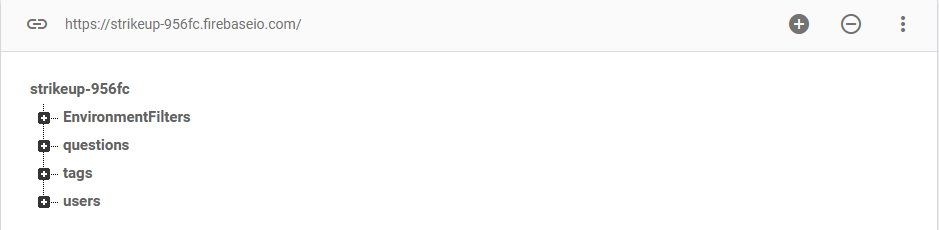
\includegraphics[width=0.85\textwidth]{db_minimiert}
    \caption{Minimierte Struktur der Datenbank}
    \label{img:db_minimiert}
\end{figure}
Daten werden in der Datenbank in Form vier verschiedener Kategorien gespeichert: \glqq{}EnvironmentFilters\grqq{} (Umgebungsvariablen), \glqq{}questions\grqq{} (Fragen),
\glqq{}tags\grqq{} (Tags) und \glqq{}users\grqq{} (Nutzer/-innen) (vgl. \ref{img:db_minimiert}).

Die Verwaltung der Datenbank erfolgt durch den Besitzer des Firebase-Projektes. Dies geschieht über eine Konsole. Um auf diese Konsole zuzugreifen, wird das entsprechende Google-Konto benötigt. \newline
Über die Konsole können in der Datenbank gespeicherte Daten beliebig geändert, gelöscht und hinzugefügt werden. Nutzerkonten können deaktiviert oder gelöscht werden. \newline
Bei einer Deaktivierung eines Nutezrkontos kann der/die entsprechende Nutzer/-in sich nicht mehr bei Strike Up anmelden. Des Weiteren kann eine Zurücksetzung des Passworts angefordert werden. \newline
Über die Konsole kann der aktuell genutzte Speicherplatz, sowie die in diesem und im vorherigen Monat heruntergeladene Datenmenge eingesehen werden. \newline
Zu den Nutzern/-innen werden (anonymisiert) das Land, in welchem sie Strike Up verwenden, das verwendete Betriebssystem, sowie die in der App verbrachte Zeit angezeigt. \newline
Außerdem können Zugriffsregeln für individuelle Abschnitte der Datenbank definiert werden.

Lese- und Schreibaufrufe werden im Code asynchron ausgeführt. Das bedeutet der Code \glqq{}läuft\grqq{} weiter, während der Lese-/Schreibaufruf im Hintergrund ausgeführt wird. Dies
verhindert das Finden von Fehlern mit einem \gls{debugger}, da Variablen, welche Daten aus der Datenbank enthalten, zur Laufzeit immer Null sind. Eine Fehlersuche im Zusammenhang mit
Leseaufrufen der Datenbank gestaltet sich somit schwierig. \newline
Wenn Daten aus der Datenbank in darauffolgendem Code benötigt werden, so muss auf die Fertigstellung des Lesevorgangs gewartet werden, da ansonsten mit Null-Objekten gearbeitet wird. Null-Objekte
würden zu Fehlern in der Anwendung führen. \newline
Ein Leseaufruf besteht aus einem \gls{listener}, welcher auf einen Knotenpunkt der Datenbank registriert wird. Beim Setzen eines \gls{listener}s (und wahlweise bei Veränderung der Daten
unter dem registrierten Knotenpunkt) wird dessen Funktion einmal ausgeführt. Um Null-Objekte zu verhindern, werden, auf einen Leseaufruf folgende, Funktionen in dem zugehörigen \gls{listener}
aufgerufen. Dies umgeht das asynchrone Ausführen der Leseaufrufe. Bei mehrern aufeinanderfolgenden Leseaufrufen, verzögert sich jedoch die Ausführung des Codes, da bei jedem Aufruf auf
dessen Fertigstellung gewartet wird. Dies kann in Extremfällen, und bei langsamem Internet, die Ausführung der App verlangsamen.


\section{Nutzerprofile}
\label{sec:profile}

Damit Nutzer/-innen Zugriff auf die von Strike Up bereitgestellten Funktionen haben, müssen sie sich zuerst registrieren. Eine Registrierung verhindert, in beschränktem Maße, dass die
von Strike Up genutzte Datenbank mit ungenutzten Nutzerprofilen gefüllt wird. Dies spart Speicherplatz, welcher im kostenlosen Vertrag beschränkt ist.
\begin{figure}[htpb]
    \centering
    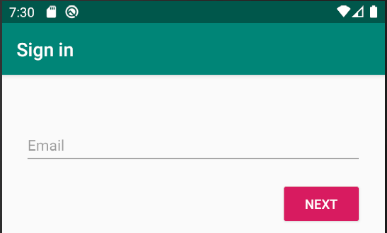
\includegraphics[width=0.5\textwidth]{Sign_in}
    \caption{Anmeldung mit E-Mail-Adresse}
    \label{img:signin_email}
\end{figure}
\begin{figure}[htpb]
    \centering
    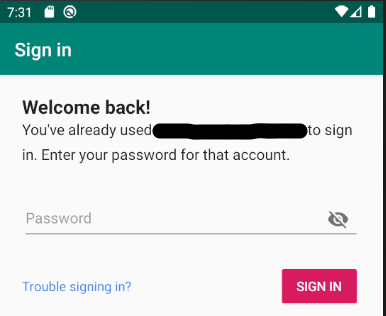
\includegraphics[width=0.5\textwidth]{sign_in_password}
    \caption{Aufforderung zur Eingabe des Passworts}
    \label{img:signin_password}
\end{figure}
Die Anmeldung erfolgt über eine E-Mail-Adresse und ein Passwort (siehe \ref{img:signin_email} und \ref{img:signin_password}). Ist die E-Mail-Adresse bereits auf ein Konto registriert, so
wird der/die Nutzer/-in aufgefordert das dazugehörige Passwort einzugeben (\ref{img:signin_password}). Wenn mit der E-Mail-Adresse ein neues Konto angelegt wird, so muss der/die Nutzer/-in
ein neues Passwort für diesen Account festlegen.

In der Datenbank werden Nutzer/-innen unter ihrer \gls{uid} gespeichert. Die \gls{uid} ist eine einzigartige, von Firebase automatisch generierte Kennung. Anhand dieser einzigartigen
Kennung wird jede/-r Nutzer/-in von Strike Up identifiziert. Wird eine Nutzeraccount gelöscht, so wird auch dessen \gls{uid} entfernt.

Abgesehen von der \gls{uid} besitzt ein Nutzerprofil folgende Attribute:
\begin{itemize}
    \item Name: Der Name des/der Nutzers/-in
    \item Email: Die E-Mail-Adresse des/der Nutzers/-in
    \item Alter: Das Alter des/der Nutzers/-in
    \item PreferredTags: Eine Liste aller Tags, welche der/die Nutzer/-in bevorzugt
    \item IgnoredTags: Eine Liste aller Tags, welche der/die Nutzer/-in vermeiden will
    \item ConversationalPartners: Eine Liste aller gespeicherten Gesprächspartner/-innen (siehe \ref{subsec:gespraechspartner}) des/der Nutzers/-in
\end{itemize}


\subsection{Tags}
\label{subsec:tags}

Tags werden in der Datenbank unter dem Knoten \glqq{}tags\grqq{} gespeichert. Ein Tag besitzt keine Attribute. Tags sind für jeden authentifizierten Nutzer einsehbar.

Nutzer/-innen wählen aus der Liste aller verfügbaren Tags aus, ob ihnen ein Tag gefällt oder nicht. Das Auswählen der bevorzugten und gemiedenen Tags geschieht dabei über zwei separate
Buttons. \newline
Tags, welche bereits in der Liste bevorzugter Tags sind, werden beim Hinzufügen neuer bevorzugter Tags nicht mehr zur Auswahl angeboten. Das Gleiche gilt für gemiedene Tags. Beim Hinzufügen
neuer bevorzutger Tags werden jedoch auch Tags angezeigt, welche in der Liste gemiedener Tags vorhanden sind. Dies gilt auch umgekehrt. \newline
\begin{figure}[htpb]
    \centering
    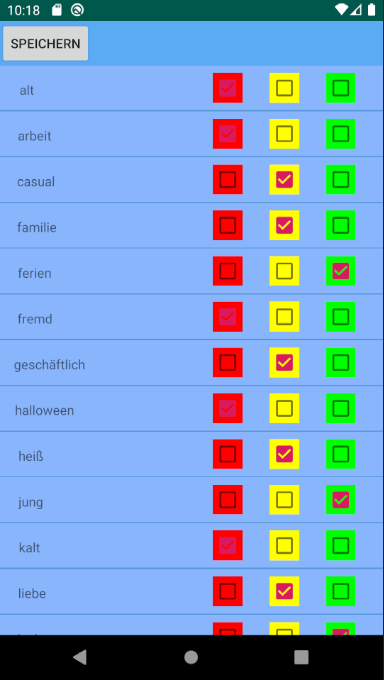
\includegraphics[width=0.35\textwidth]{alle_tags}
    \caption{Auswahl bevorzugter und gemiedener Tags}
    \label{img:alle_tags}
\end{figure}
Damit Tags nur in einer Liste vorkommen, und um die Auswahl der Tags zu vereinfachen, wird eine neue Funktion entwickelt, welche über mehrere Checkboxen das Aufteilen der Tags in die
entsprechenden Listen ermöglicht (\ref{img:alle_tags}). Rot steht dabei für gemiedene Tags und grün für bevorzugte Tags. Gelb markierte Tags sind in keiner der beiden Listen vorhanden und werden somit neutral bewertet. \newline
Ein Problem tut sich dabei bei der Implementation einer \gls{listactivity} in Android auf. Da mehr Objekte in der anzuzeigenden Liste sind, als auf den Bildschirm passen, verwendet Android
bereits für angezeigte Elemente verwendete \gls{container}, um noch nicht angezeigte Elemente zu laden \cite{misc:android_listview}. Das bedeutet: Wenn ein, mit einem Objekt gefüllter,
\gls{container} (durch scrollen) vom Bildschirm verschwindet, wird dieser \gls{container} benutz um das neu erschienene Element anzuzeigen. Der \gls{container} behält dabei die
Position des Hakens der Checkbox. Beim Scrollen, wird somit bei neu erschienen Tags der Haken an der Position der neu ausgeblendeten Tags gesetzt. Dies lässt sich durch das Verwenden
einer \gls{hashmap}, welche die Positionen der Haken speichert, umgehen. Dabei ist der Name eines Tags der \glqq{}Key\grqq{} und die Position des Hakens das \glqq{}Value\grqq{}. \newline
Aus Zeitgründen ist diese Funktion noch nicht fehlerfrei lauffähig. Deshalb geschieht die Auswahl bevorzugter und gemiedener Tags weiterhin über zwei separate Buttons.

Während der Entwicklung wurden Tags um eine ID erweitert; Tags werden somit unter ihrer ID gespeichert und besitzen das Attribut \glqq{}Name\grqq{}. \newline
Das Verwenden einer ID ermöglicht, dass Strike Up auf weitere Sprachen erweitert werden kann. So können Tags beispielsweise um die Attribute \glqq{}Name-en\grqq{} oder \glqq{}Name-fr\grqq{} erweitert
werden.

\subsection{Gesprächspartner/-innen}
\label{subsec:gespraechspartner}

Gesprächspartner/-innen werden als eine, zu einem/-r Nutzer/-in gehörende, Liste gespeichert. Jede/-r Nutzer/-in kann beliebig viele Gesprächspartner/-innen hinzufügen. \newline
Ein/-e Gesprächspartner/-in besitzt die Attribute:
\begin{itemize}
    \item Name: Name des/der Gesprächspartners/-in
    \item Gender: Geschlecht des/der Gesprächspartners/-in
    \item Alter: Alter des/der Gesprächspartners/-in
    \item IgnoredTags: Eine Liste aller Tags, welche der/die Gesprächspartner/-in vermeiden will
    \item PreferredTags: Eine Liste aller Tags, welche der/die Gesprächspartner/-in bevorzugt
    \item Notizen: Von dem/der Nutzer/-in verfasste Notizen zu dem/der Gesprächspartner/-in
\end{itemize}
Das Bearbeiten und Auswählen von Tags geschieht dabei gleich wie bei einem/-r Nutzer/-in.

Gesprächspartner/-innen werden um das Atttribut ID erweitert, da sie bisher unter ihrem Namen in der Datenbank gespeichert wurden. Das Speichern unter dem Namen erzeugte Probleme, wenn
der Name geändert wurde, da so zwei Objekte desselben Partnerprofils in der Datenbank hinterlegt waren. Gebraucht wird aber nur ein Objekt. Es entsanden also redundante Daten. \newline
Das Einführen einer unveränderlichen und einzigartigen ID ermöglicht eine problemfreie Änderung des Namens. \newline
Die ID wird von Firebase generiert. Zum erstellen dieser einzigartigen ID benutzt Firebase den gewünschten Speicherort innerhalb der Datenbank und das aktuelle Datum.

Nachdem das Profil eines/-r Gesprächspartners/-in erstellt ist, kann dieses bearbeitet und wieder gelöscht werden.

Strike Up besitzt individuelle Profile für den/die Nutzer/-in und für Gesprächspartner/-innen. Somit ist F-6 erfüllt (vgl. \ref{tab:funktional}).


\section{Fragen/Hinweise}
\label{sec:fragen_hinweise}

Fragen und Hinweise werden in der Datenbank unter \glqq{}questions\grqq{} gespeichert. Eine einzelne Frage ist dabei unter ihrer ID zu finden. \newline
Fragen besitzen folgende Attribute:
\begin{itemize}
    \item ID: Eine eindutige ID, unter welcher die Frage gespeichert ist
    \item tags: Eine Liste aller Tags, welche zu dieser Frage passen
    \item text: Der Text der Frage
\end{itemize}
Fragen und Hinweise können nicht von Nutzern/-innen bearbeitet werden. Das Verändern, Hinzufügen und Entfernen von Fragen obliegt somit dem/der Verwalter/-in der Datenbank. \newline
Ursprünglich war geplant, dass Nutzer/-innen sowohl Fragen als auch Tags zur Datenbank hinzufügen können, da die Datenbank besonders in den Anfängen von Strike Up noch nicht vollständig
ist. Diese Idee wurde jedoch aus Angst vor Missbrauch wieder gestrichen.

\subsection{Umgebungsvariablen}
\label{subsec:umgebungsvariablen}

Eine Umgebungsvariable wird mit folgenden Attributen in der Datenbank gespeichert:
\begin{itemize}
    \item ID: Eine eindutige ID, unter welcher die Umgebungsvariable gespeichert ist
    \item Name: Der Name der Umgebungsvariable
    \item IgnoredTags: Liste aller Tags, auf welche die Umgebungsvariable einen negativen Einfluss hat
    \item Preferred Tags: Liste aller Tags, auf welche die Umgebungsvariable einen positiven Einfluss hat
\end{itemize}
Umgebungsvariablen werden vor einem Gepräch entweder automatisch generiert oder durch den/die Nutzer/-in gesetzt. \newline
Die Umgebungsvariable Alter (jung/alt) wird automatisch generiert und der/die Nutzer/-in kann die Umgebungsvariable \glqq{}Privat\grqq{} oder \glqq{}Geschäftlich\grqq{}
auswählen. Alternativ kann die Auswahl einer Umgebungsvariable auch übersprungen werden. \newline
Das automatische Generieren und manuelle Auswählen von Umgebungsvariablen ist noch erweiterbar. Die bisherige Implementation stellt einen konzeptionellen Beweiß der Erfüllbarkeit von F-13 dar.

Im Laufe der Arbeit kam auf, dass die Eingabe eines statischen Alters bei Nutzerprofilen und Gesprächspartnern/-innen nicht sinnvoll ist, da sich dieses jährlich ändert.
Fragen und Hinweise beziehen sich auf das Alter und Strike Up setzt automatisch Umgebungsvariablen zu diesem (z.B. Jung oder Alt). Aus diesem Grund wird Alter als Profil-Attribut entfernt.
Stattdessen wird das Geburtsdatum verwendet. Aus diesem wird, bei einem Datenbankabruf des Profils, das Alter ermittelt. Somit aktualisiert sich das Alter eines Profils am Geburtstag.


\section{Gespräch}
\label{sec:gespräch}

Vor einem Gespräch wird aus der Liste aller verfügbaren Gesprächspartner/-innen ein/-e Gesprächspartner/-in ausgewählt oder alternativ ein/-e neue/-r Gesprächspartner/-in erstellt.
Anschließend kann der/die Gesprächspartner/-in noch einmal bearbeitet werden. Bevor die Konversation beginnt wählt der/die Nutzer/-in noch manuell Umgebungsvariablen aus.

Die Listen bevorzugter Tags des/der Nutzers/-in, des Gegenübers und der Umgebungsvariablen werden addiert. Doppelte (dreifache, vierfache, \dots) Tags sind dabei erlaubt. Das Gleiche passiert
mit den entsprechenden Listen gemiedener Tags. \newline
Ist die Listen fertig, so wird diese mit den entsprechenden Listen jeder verfügbaren Frage verglichen. Hierfür werden alle Tags der bevorzugten/gemiedenen Listen einzeln
miteinander verglichen. \newline
Kommt ein Tag sowohl in der Liste der bevorzugten (gemiedenen) Tags einer Frage, als auch in der kombinierten Liste bevorzugter Tags von Nutzers/-in, Gegenüber und Umgebungsvariablen vor,
so wird bei der Frage ein Punkt addiert (subtrahiert). Fragen starten dabei mit einer Punktzahl von null.

\begin{figure}[htpb]
    \centering
    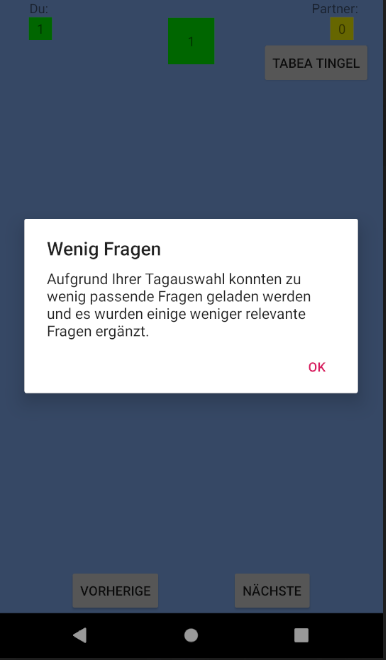
\includegraphics[width=0.35\textwidth]{warning_conversation}
    \caption{Warnung, wenn weniger relevante Fragen hinzugefügt werden}
    \label{img:warning_conversation}
\end{figure}

Für die Konversation werden nur Fragen mit einer Punktzahl über null ausgewählt. Sollten somit jedoch weniger als zehn Fragen verfügbar sein, so werden auch Fragen mit einer Punktzahl von null
hinzugefügt. Sind immer noch weniger als zehn Fragen vorhanden, so werden auch negativ bewertete Fragen hinzugefügt. Der/die Nutzer/-in wird durch ein \gls{popup} auf diesen Umstand aufmerksam gemacht
(vgl. \ref{img:warning_conversation}).

Während einem Gespräch sieht die \gls{ui} wie in \ref{img:conversation} aus. Über die Buttons \glqq{}vorherige\grqq{} und \glqq{}nächste\grqq{} kann zwischen den für das Gespräch
verfügbaren Fragen gewechselt werden (F-5). Der Text der Fragen wird zentral im Bildschirm angezeigt, während andere Funktionen, wie Buttons, am Rand vorhanden sind (NF-3).
\begin{figure}[htpb]
    \centering
    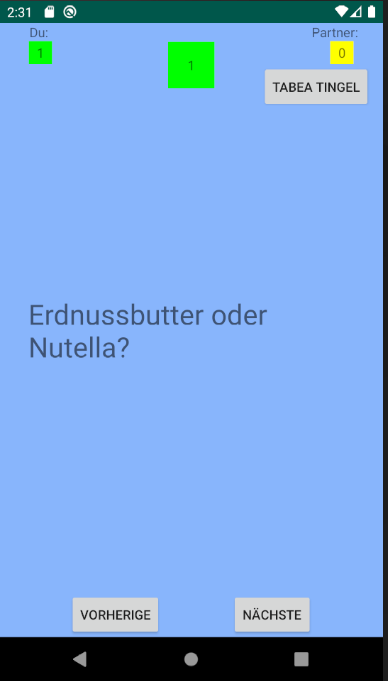
\includegraphics[width=0.35\textwidth]{conversation}
    \caption{Frage während einer Konversation}
    \label{img:conversation}
\end{figure}
Das farbige Quadrat unter \glqq{}Du\grqq{} zeigt die Bewertung der Frage aus Sicht des Nutzers an. Das Quadrat unter \glqq{}Partner\grqq{} zeigt die Bewertung aus Sicht des Gegenübers
und das große Quadrat zeigt die Gesamtbewertung. Eine grüne Farbe steht dabei für eine positive, gelb für eine neutrale und rot für eine negative Bewertung.

Über \glqq{}Tabea Tingel\grqq{} wird das Profil des Gegenübers aufgerufen. Somit sind Notizen des Gegenübers während einem Gespräch verfügbar (F-7). Das Profil des/der Gesprächspartners/-in
kann somit auch erst während einer Konversation mit Informationen befüllt werden.


\section{Datenschutz}
\label{sec:datenschutz}

Strike Up soll keine personenbezogenen Daten an Dritte weitergeben (vgl. \ref{tab:nichtfunktional}, NF-4). Als \glqq{}Dritte\grqq{} ist hierbei Google in der Rolle des Verwalter der Daten,
zu verstehen. \newline
Google ist hierbei ein \glqq{}processor of [...] Customer Personal Data under the European Data Protection Legislation\grqq{} \cite{misc:firebase_terms}. Dies bedeutet, dass Google ein
Verwalter der Daten ist, diese aber nicht einsehen oder versenden darf. \newline
Da die zu Strike Up gehörende Datenbank von der EU aus bearbeitet wird, gilt die \gls{dsgvo}. Somit muss Google Daten an Behörden weiterleiten, falls dies gefordert wird.

Des Weiteren ist der Ersteller von Strike Up für das Einhalten der \gls{dsgvo} verantwortlich. Um dies zu garantieren wird beim ersten Öffnen der Anwendung ein Dialogfenster geöffnet,
welches den/die nutzer/-in auffordert zu bestätigen, dass er/sie über 18 Jahre alt ist. Außerdem willigt er/sie ein, dass alle von Strike Up verarbeiteten Daten gespeichert werden. \newline
Wird eine dieser zwei Bedienungen nicht erfüllt, so schließt sich Strike Up und der Ablauf wird beim nächsten Öffnen wiederholt.

\subsection{Schutz vor Datendiebstahl}
\label{subsec:datendiebstahl}

Damit Strike Up auf die Cloud-Datenbank zugreifen kann, wird eine \gls{url} zu dieser benötigt. Die \gls{url} ist dabei im Code der Anwendung enthalten. \newline
Diese \gls{url} ermöglicht Angreifern jedoch keinen Zugriff auf die Datenbank, da zudem noch das verbundene Google-Konto benötigt wird.

Eine weitere Angriffsmöglichkeit ist der im Quellcode hinterlegte \gls{api}-Key, welcher Strike Up bei der Datenbank registriert. Über den \gls{api}-Key können Angreifer auf alle in der
Datenbank gespeicherten Daten zugreifen. \newline
Dies wird durch das Aufstellen von Regeln verhindert. Regeln beziehen sich auf definierte Bereiche der Datenbank. Die für Strike Up definierten Regeln erlauben
jedem/-r authentifizierten Nutzer/-in das Lesen der Bereiche \glqq{}EnvironmentFilters\grqq{}, \glqq{}questions\grqq{} und \glqq{}tags\grqq{} (vgl. \ref{img:db_minimiert}). \newline
Da der Bereich \glqq{}users\grqq{} nutzerspezifische Daten enthält, ist nicht jedem/-r Nutzer/-in erlaubt alle darunter liegenden Knoten zu lesen. Jede/-r Nutzer/-in kann dabei nur auf
\glqq{}unter\grqq{} seiner/ihrer \gls{uid} gespeicherte Daten zugreifen. Der/die Nutzer/-in hat für diesen Bereich Lese- und Schreibrechte.
\chapter{Praxistests}
\label{ch.praxistests}

Strike Up soll Menschen beim Eröffnen und Führen von Gesprächen helfen (\ref{sec:vision}). Um die Wirksamkeit diser Hilfestellungen zu testen, wurden mit der entwickelten Applikation Praxistests durchgeführt. \newline
Gesprächspartner/-innen waren dabei zufällige Passanten auf der Straße und in Drogeriemärkten. \newline
Die folgenden Erkenntnisse beruhen auf empirischen Erfahrungen.

Während den Tests erwies sich besonders das Vorbereiten auf das Gespräch als hilfreich. Präparierte Gesprächsthemen halfen dabei, eine Konversation interessant zu gestalten und am Laufen zu halten. \newline
Da die Versorgung mit Gesprächsthemen durch Strike Up aus zeitlichen Gründen in dieser Arbeit nicht zureichend entwickelt wurde, wurden externe Quellen (News-Webseiten, Nachrichten im Fernesehen) hinzugezogen. Mit diesen Quellen
wurde das von Strike Up gewünschte Verhalten nach F-9 und F-10 simuliert.

Auf sich selbst und das Gegenüber angepasste Fragen erwiesen sich als vergleichsweise durchschnittlich nützlich. Fragen entstanden eher spontan und aus den bereits vorbereiteten Themn heraus. \newline
Das Vermeiden unpassender Fragen hingegen sorgte dafür, dass für sich selbst und das Gegenüber unangenehme Themen nicht angesprochen wurden. Dies verhinderte einen abrupten Abbruch der Konversation.

Eine unerwartete Entdeckung war, dass das Gegenüber, wenn es die Zuhilfenahme der App bemerkte, meist positiv mit einem Lachen reagierte. Als Grund für das Lachen wurde genannt, dass das Verwenden der App den/die Benutzer/-in sympathisch darstelle. Der/die Nutzer/-in würde eine Schwäche einsehen und versuche diese zu verbessern. \newline
Es kamen aber auch Fälle vor, bei welchen sich das Gegenüber ablenend gegenüber der App äußerte und das Gespräch somit beendete. Das Smartphone würde dabei dem/der Nutzer/-in die Konversationsführung wegnehmen und somit zu einer Verdummung führen.

Es wurde aber auch festgestellt, dass Strike Up um eine Schnellgespräch-Funktion erweitert werden sollte. \newline
Will der/die Nutzer/-in spontan ein Gespräch beginnen, so muss zuerst ein/-e Gesprächspartner/-in ausgewählt werden und anschließend Umgebungsvariablen gesetzt werden. Dieser Prozess kann, besonders beim Erstellen eines/-r neuen Gesprächspartners/-in Zeit in Anspruch nehmen. \newline
Um diesen Prozess zu umgehen, kann im Hauptbildschirm ein Button hinzugefügt werden, welcher sofort ein Gespräch startet. Die \gls{ui} des Gespräches entspricht dabei der \gls{ui} einer normalen Konversation. Das Profil des/der Gesprächspartners/-in wird während der Konversation entdeckt/erstellt.
\chapter{Zusammenfassung}
\label{ch:zusammenfassung}

Mit dieser Arbeit sollte ein kontextabhähniger Kommunikationsassistent entwickelt werden (\ref{sec:vision}). Dies wurde in Form einer Applikation namens Strike Up umgesetzt.

Strike Up ist eine für Android entwickelte App, welche dem/der Nutzer/-in ermöglicht ein eigenes Profil, sowie Profile von Gesprächspartnern/-innen, zu erstellen. Diese Profile enthalten bevorzugte und gemiedene Tags, anhand welcher während einer Konversation Fragen ausgewählt und vorgeschlagen werden. Des Weiteren haben automatisch generierte und durch den/die Nutzer/-in ausgewählte Umgebungsvariablen einen Einfluss auf die Auswahl der Fragen. \newline
Fragen beziehen sich somit auf bevorzugte und weniger bevorzugte Themen des/der Nutzers/-in und des Gegenübers, sowie auf die Umgebung der Konversation.

Um Strike Up nutzern zu können, müssen sich Nutzer/-innen mit einer E-Mail-Adresse und einem Passwort anmelden. Anschließend wird eine Altersbestätigung, sowie eine Einwilligung zur Speicherung der Daten gefordert.

Jegliche von Strike Up zur Verfügung gestellte, sowie durch den/die Nutzer/-in erstellte, Daten werden in der, von Google gehosteten, Cloud-Datenbank Firebase gespeichert. Nutzer/-innen können dabei alle Teile der Datenbank lesen, welche keine Informationen anderer Nutzer/-innen enthalten. Schreibzugriffe werden Nutzern/-innen nur bei selbst erstellten Daten (eigenes Profil, Gesprächspartner/-innen) gestattet.

Als besonders interessant haben sich die im Zuge dieser Arbeit durchgeführten Praxistests erwiesen. \newline
Die zufällig ausgewählten Gesprächspartner/-innen reagierten meist positiv auf das Verwenden einer App als Hilfestellung und fanden dies sogar sympathisch. \newline
Während einem Gespräch hat sich dabei die Vorbereitung auf das Gespräch als am hilfreichsten erwiesen. Weniger hilfreich war die Auswahl bevorzugter Fragen. Hierbei hat sich das Ausschließen unpassender Fragen als nützlicher erwiesen.
\chapter{Ausblick}
\label{ch:ausblick}

Bevor Strike Up im Google Play Store, oder firmenintern, veröffentlicht werden kann, müssen noch einige Features verbessert werden: Die Benutzeroberfläche sollte ansprechender werden
und das editieren von Tags könnte, für eine bessere Übersicht, in einem (statt zwei verschiedenen) Bildschirm stattfinden. \newline
Fragen und Hinweise können noch nicht durch den/die Nutzer/-in bewertet werden und ein Feedback am Ende eines Gespräches ist auch nicht vorhanden (vgl. \ref{tab:funktional}, F-2, F-4, F-10).
Des Weiteren können Fragen noch nicht aus der Auswahl ausgeschlossen werden (F-3). Auch die Versorgung mit aktuellen Themen, beispielsweise durch einen \gls{rssfeed}, wurde nicht umgesetzt (F-8, F-9).
Es gibt auch keine einfache Funktion, mit welcher ein/-e Nutzer/-in sein/ihr Konto und damit verbundene Daten löschen kann (F-11). Dies ist möglich, indem der Verwalter der Datenbank kontaktiert wird,
jedoch ist diese Funktion nicht in Strike Up intgriert.

In der aktuellen Form kann Strike Up noch in viele Richtungen verbessert und erweitert werden: Die Gesprächsunterstützung könnte von einer Unterstützung bei One-on-One-Gesprächen auf
eine Unterstützung während Gruppengesprächen und Diskussionen erweitert werden. \newline
Das Bewerten von Fragen kann durch ein Fragen-Rating, ähnlich wie bei der Fragenbewertung vor einem Gespräch, ermöglicht werden. \newline
Nutzer/-innen könnten, durch drücken eines Buttons, die aktuell vorgeschlagene Frage in eine Liste ignorierter Fragen setzen. Vor einem Gespräch würden, für die Konversation vorgeschlagene, Fragen
mit der Liste der ignorierten Fragen verglichen werden. Wenn eine Fragen in beiden Listen vorkommt, so würde diese nicht während dem Gespräch vorgeschlagen werden. \newline
Strike Up könnte während einer Konversation Fragen als Push-Benachichtigung anzeigen. Somit müsste das Smartphone zum Einsehen einer Frage nicht mehr entsperrt werden. \newline
Die App kann um eine Vorlese-Funktion erweitert werden. Fragen werden dem/der Nutzer/-in über Kopfhörer vorgelesen. Mit den Kopfhörerfunktionen (überspringen, zurück) könnte zwischen Fragen
gewechselt werden. \newline
Des Weiteren könnte der aktuelle Standord benutzt werden um auf Attraktionen in der Nähe hinzuweisen oder um Wetterinformationen abzurufen. Die Wetterinformationen könnten dabei über
OpenWeather \cite{misc:openweather} abgerufen werden. \newline
Strike Up kann über eine zusätzliche App für Smartwatches erweitert werden. Während einem Gespräch könnten somit Fragen und Hinweise auf der Smartwatch angezeigt werden und das Smartphone
bliebe somit in der Tasche.

\appendix
\chapter[Anhang]{}
\label{ch:anhang}

\lstdefinelanguage{WinDbg}{
   alsoletter={., |, +, :, 0, >, !, ?},
   keywords=[1]{.time, .exr, .sympath, .sympath+, .symfix, .symfix+, .symopt, .symopt+, |, ||, .reload, lm, !sym, k, .excr, .ecxr, .thread, .cxr, .frame, dv, dD, dx, dq, ?},
   keywordstyle=[1]\color{dkgreen},
   keywords=[2]{0:000>},
   keywordstyle=[2]\color{gray},
   sensitive=false, % keywords are not case-sensitive
   morecomment=[l]{}, % l is for line comment
   morecomment=[s]{/*}{*/}, % s is for start and end delimiter
   morestring=[b]" % strings are enclosed in double quotes
} % 
\lstset{language=WinDbg}

\section{WinDbg Crash Analyse}
\label{sec:windbg}
Vom betroffenen Absturz, der womöglich auf Undefined Behavior zurückzuführen ist, wurde ein Crash Dump erstellt.
Dieser Anhang beschreibt anhand einer aufgezeichneten Logdatei, welche Befehle genutzt wurden, um den Crash Dump zu analysieren.
Bei der analysierten Datei handelt es sich um einen Crash Dump mit vollständig enthaltenem Speicherinhalt. Die Datei ist ca. 1 GB groß.

Die hier beschriebene Analyse wurde von Mitarbeitern des CTL durchgeführt und für die Studienarbeit zur Verfügung gestellt.

\subsection{Grundlegende Prüfungen}
\begin{figure}[H]
\begin{lstlisting}
0:000> ||
.  0 Full memory user mini dump: D:\MINIDUMP-20201217-150359.DMP
\end{lstlisting}
\caption{Ausgabe der analysierten Datei in WinDbg}
\end{figure}

Dem Dateinamen nach wurde der Crash Dump am 17.12.2020 um 15:03:59 Uhr UTC geschrieben. Die Zeitangabe innerhalb des Crash Dumps bestätigt dies.

\begin{figure}[H]
\begin{lstlisting}
0:000> .time
Debug session time: Thu Dec 17 16:04:00.000 2020 (UTC + 1:00)
System Uptime: 0 days 7:25:08.968
Process Uptime: 0 days 0:01:31.000
  Kernel time: 0 days 0:00:32.000
  User time: 0 days 0:00:48.000
\end{lstlisting}
\caption{Ausgabe der Uhrzeit zum Zeitpunkt des Crashs in WinDbg}
\end{figure}

Der Bug wurde am 27.11.2020 berichtet und am 11.12.2020 erstmals bestätigt. Beim vorliegenden Crash Dump handelt es sich also um die Reproduktion des Fehlers zu einem späteren Zeitpunkt.

\begin{figure}[H]
\begin{lstlisting}
0:000> |
.  0	id: 2b7c	examine	name: C:\MCOSMOSx64\EXE\GEOPAK64.exe
\end{lstlisting}
\caption{Ausgabe des ausgeführten Programms in WinDbg}
\end{figure}
Das ausgeführte Programm stimmt mit dem des Fehlerberichts überein.

\begin{figure}[H]
\begin{lstlisting}[language=WinDbg]
0:000> .exr -1
*** WARNING: Unable to verify checksum for MnGeom364.dll
ExceptionAddress: 00007ff995c1d48e (MnGeom364!tg_ajc_lin_int+0x000000000000014e)
   ExceptionCode: c0000005 (Access violation)
  ExceptionFlags: 00000000
NumberParameters: 2
   Parameter[0]: 0000000000000000
   Parameter[1]: 0000000000000000
Attempt to read from address 0000000000000000
\end{lstlisting}
\caption{Abfrage der Exception in WinDbg}
\end{figure}
Der Fehlercode und das fehlerhafte Modul stimmen ebenfalls mit dem des Fehlerberichts überein. Es kann also eine detailliertere Analyse durchgeführt werden.

\subsection{Symbole}
Für eine weitere Analyse ist das Vorhandensein von Symbolen erforderlich. Manche Symbole wurden zusammen mit dem Crash Dump abgelegt.
Diese Symbole sollten zuerst berücksichtigt werden und müssen zuerst in den Symbolpath aufgenommen werden.
\begin{figure}[H]
\begin{lstlisting}[language=WinDbg]
0:000> .sympath "D:\temp\Bug 32147"
Symbol search path is: D:\temp\Bug 32147
Expanded Symbol search path is: d:\temp\bug 32147

************* Path validation summary **************
Response                         Time (ms)     Location
OK                                             D:\temp\Bug 32147
\end{lstlisting}
\caption{Einstellen des Pfades zu Symboldateien in WinDbg}
\end{figure}

Leider stimmen bei den Symbolen die Zeitstempel nicht überein, so dass die Symbole nicht geladen werden können.
Die Prüfung des Zeitstempels kann jedoch ausgeschaltet werden.
\begin{figure}[H]
\begin{lstlisting}[language=WinDbg]
0:000> .symopt+ 0x40
Symbol options are 0x30377:
  0x00000001 - SYMOPT_CASE_INSENSITIVE
  0x00000002 - SYMOPT_UNDNAME
  0x00000004 - SYMOPT_DEFERRED_LOADS
  0x00000010 - SYMOPT_LOAD_LINES
  0x00000020 - SYMOPT_OMAP_FIND_NEAREST
  0x00000040 - SYMOPT_LOAD_ANYTHING
  0x00000100 - SYMOPT_NO_UNQUALIFIED_LOADS
  0x00000200 - SYMOPT_FAIL_CRITICAL_ERRORS
  0x00010000 - SYMOPT_AUTO_PUBLICS
  0x00020000 - SYMOPT_NO_IMAGE_SEARCH
\end{lstlisting}
\caption{Abschalten der Prüfung von Zeitstempel und Hash in WinDbg}
\end{figure}

Weitere Symbole können vom Azure DevOps Server geladen werden
\begin{figure}[H]
\begin{lstlisting}[language=WinDbg]
0:000> .sympath+ srv*d:\debug\symbols*\\tfs-build-2014\SymbolStore\Mitutoyo.MCOSMOS.BasicLibs_Release_NuGet
Symbol search path is: D:\temp\Bug 32147;srv*d:\debug\symbols*\\tfs-build-2014\SymbolStore\Mitutoyo.MCOSMOS.BasicLibs_Release_NuGet
Expanded Symbol search path is: d:\temp\bug 32147;srv*d:\debug\symbols*\\tfs-build-2014\symbolstore\mitutoyo.mcosmos.basiclibs_release_nuget

************* Path validation summary **************
Response                         Time (ms)     Location
OK                                             D:\temp\Bug 32147
Deferred                                       srv*d:\debug\symbols*\\tfs-build-2014\SymbolStore\Mitutoyo.MCOSMOS.BasicLibs_Release_NuGet
\end{lstlisting}
\caption{Einstellen eines Symbolstores auf einem Netzlaufwerk in WinDbg}
\end{figure}

Und letztlich muss der Microsoft Server abgefragt werden, damit die Funktionen des Betriebssystems korrekt aufgelöst werden können.
\begin{figure}[H]
\begin{lstlisting}[language=WinDbg]
0:000> .symfix+ d:\debug\symbols
\end{lstlisting}
\caption{Einstellen des Microsoft Symbol Servers in WinDbg}
\end{figure}


Nach dem Ändern der möglichen Quellen für Symbole muss dem Debugger mitgeteilt werden, dass er seine Informationen aktualisiert.

\begin{figure}[H]
\begin{lstlisting}
0:000> .reload /f
.*** WARNING: Unable to verify checksum for GEOPAK64.exe
.......*** WARNING: Unable to verify checksum for GeoWinBinToAsc64.dll
.....*** WARNING: Unable to verify checksum for Mafis_3DCmp64.dll
.......*** WARNING: Unable to verify checksum for MnGeoWnListCtrl64.dll
.*** WARNING: Unable to verify checksum for MnRecordPoints64.dll
.*** WARNING: Unable to verify checksum for UncertaintyCalculator64.dll
..

Press ctrl-c (cdb, kd, ntsd) or ctrl-break (windbg) to abort symbol loads that take too long.
Run !sym noisy before .reload to track down problems loading symbols.

[...]
Loading unloaded module list
..........................

************* Symbol Loading Error Summary **************
Module name            Error
WkWin64                The system cannot find the file specified
GeoWinBinToAsc64       The system cannot find the file specified
[...]

You can troubleshoot most symbol related issues by turning on symbol loading diagnostics (!sym noisy) and repeating the command that caused symbols to be loaded.
You should also verify that your symbol search path (.sympath) is correct.
\end{lstlisting}
\caption{Erneutes Einlesen von Symbolen in WinDbg}
\end{figure}

Anhand der beiden bekannten und für die Fehleranalyse notwendigen Module \verb|Geopak| und \verb|MnGeom3| kann überprüft werden, ob die Symbole korrekt geladen wurden.

\begin{figure}[H]
\begin{lstlisting}
0:000> lm m geopak*
Browse full module list
start             end                 module name
00007ff7`fa2d0000 00007ff7`fc142000   GEOPAK64 C (private pdb symbols)  d:\temp\bug 32147\GEOPAK64.pdb

0:000> lm m mngeom364
Browse full module list
start             end                 module name
00007ff9`95c00000 00007ff9`95c2c000   MnGeom364 C (private pdb symbols)  d:\temp\bug 32147\MnGeom364.pdb
\end{lstlisting}
\caption{Ausgabe von Informationen zu Symbolen ausgewählter Module in WinDbg}
\end{figure}

Für beide Module sind Symbole mit Informationen zu privaten Methoden etc. vorhanden.

\subsection{Exception Analyse}

Wie bereits bei den grundlegenden Prüfungen gesehen, handelt es sich beim Absturz um eine Access Violation, also eine Art NullPointerException. Nach dem Einstellen der Symbole verschwindet allerdings die Warnung.

\begin{figure}[H]
\begin{lstlisting}
0:000> .exr -1
ExceptionAddress: 00007ff995c1d48e (MnGeom364!tg_ajc_lin_int+0x000000000000014e)
   ExceptionCode: c0000005 (Access violation)
  ExceptionFlags: 00000000
NumberParameters: 2
   Parameter[0]: 0000000000000000
   Parameter[1]: 0000000000000000
Attempt to read from address 0000000000000000
\end{lstlisting}
\caption{Erneute Abfrage der Exception nach dem Einstellen der Symbole in WinDbg}
\end{figure}

Der Callstack liefert nicht die richtigen Angaben

\begin{figure}[H]
\begin{lstlisting}
0:000> k
 # Child-SP          RetAddr               Call Site
00 00000056`12337058 00000193`813b1bec     ntdll!NtGetContextThread+0x14
01 00000056`12337060 0000001f`00000002     0x00000193`813b1bec
02 00000056`12337068 0000003e`0000003e     0x0000001f`00000002
03 00000056`12337070 00009c67`02cb62cf     0x0000003e`0000003e
04 00000056`12337078 00009c67`02cb7d3f     0x00009c67`02cb62cf
05 00000056`12337080 00000000`00000000     0x00009c67`02cb7d3f
\end{lstlisting}
\caption{Callstack im falschen Kontext in WinDbg}
\end{figure}

Dies bedeutet, dass der Kontext noch nicht auf die Exception gesetzt ist.

\begin{figure}[H]
\begin{lstlisting}
0:000> .ecxr
rax=0000000000000000 rbx=000000561233b3f8 rcx=000000561233af18
rdx=ffffffffffffffe0 rsi=000000561233b490 rdi=000000561233b470
rip=00007ff995c1d48e rsp=000000561233afe0 rbp=000000561233b0e0
 r8=00000193a1a21c90  r9=0000000000000014 r10=000000000000003c
r11=000000561233afd0 r12=00000193a1a21c90 r13=000000561233b608
r14=0000000000000014 r15=0000000000000001
iopl=0         nv up ei pl nz na pe nc
cs=0033  ss=002b  ds=002b  es=002b  fs=0053  gs=002b             efl=00010202
MnGeom364!tg_ajc_lin_int+0x14e:
00007ff9`95c1d48e 0f1000          movups  xmm0,xmmword ptr [rax] ds:00000000`00000000=????????????????????????????????
\end{lstlisting}
\caption{Ändern des Kontext auf die Exception in WinDbg}
\end{figure}

Nach dem Setzen des Kontexts wird die Methode \verb|tg_ajc_lin_int| auf dem Stack erkannt.

\begin{figure}[H]
\begin{lstlisting}
0:000> k Lb
  *** Stack trace for last set context - .thread/.cxr resets it
 # Child-SP          RetAddr               Call Site
00 00000056`1233afe0 00007ff9`95c1d8b8     MnGeom364!tg_ajc_lin_int+0x14e [d:\gitrepos\mitutoyo.mcosmos.basicslibs\source\mngeom3\tg_geom.c @ 955] 
01 00000056`1233b350 00007ff9`95c1fefb     MnGeom364!tg_ajc_lin_rl+0xd8 [d:\gitrepos\mitutoyo.mcosmos.basicslibs\source\mngeom3\tg_geom.c @ 993] 
02 00000056`1233b560 00007ff7`fae310df     MnGeom364!tg_inn_ajc_lin+0x2b [d:\gitrepos\mitutoyo.mcosmos.basicslibs\source\mngeom3\tg_geom.c @ 1026] 
03 00000056`1233b6b0 00007ff7`fae4a291     GEOPAK64!pel_line+0x77f [g:\git\mcosmos50\geopak\source\geopak\pelmadcp.cpp @ 5498] 
04 00000056`1233bf00 00007ff7`fae49687     GEOPAK64!pelm_comp_elem_intern+0xc01 [g:\git\mcosmos50\geopak\source\geopak\pelmadcp.cpp @ 8255] 
05 00000056`1233e730 00007ff7`fa7f5a88     GEOPAK64!pelm_comp_elem+0x77 [g:\git\mcosmos50\geopak\source\geopak\pelmadcp.cpp @ 8651] 
06 00000056`1233e790 00007ff7`fa920b77     GEOPAK64!fctctr_cpnt_end+0x748 [g:\git\mcosmos50\geopak\source\geopak\fctctrmngr.cpp @ 1376] 
07 00000056`1233efe0 00007ff7`fa91d26c     GEOPAK64!fctmngr_wrk_fct+0x1177 [g:\git\mcosmos50\geopak\source\geopak\fct_mngr.cpp @ 1314] 
08 00000056`1233f070 00007ff7`faaf8df3     GEOPAK64!fctmngr_wrk+0x68c [g:\git\mcosmos50\geopak\source\geopak\fct_mngr.cpp @ 1924] 
09 00000056`1233f120 00007ff7`fabd9301     GEOPAK64!CGeopakDoc::PartProgCmdWrk+0x13 [g:\git\mcosmos50\geopak\source\geopak\geopakdoc.cpp @ 3711] 
0a 00000056`1233f150 00007ff9`ab5287f9     GEOPAK64!CMainFrame::OnMsgNvUserEvent+0x281 [g:\git\mcosmos50\geopak\source\geopak\mainfrm.cpp @ 2215] 
\end{lstlisting}
\caption{Callstack im Kontext der Exception in WinDbg}
\end{figure}

Ausgehend von einer Nutzerinteraktion (\verb|OnMsgNvUserEvent|) werden mehrere Methoden aufgerufen, die dann zum Absturz führen.

\subsection{Extraktion von Daten für einen Unit Test}

Der Code der betroffenen Stelle aus \verb|TG_GEOM.C|, Commit \verb|bb882af1|.

\begin{figure}[H]
\begin{lstlisting}[language=C, numbers=left, firstnumber=937]
INTERN  MinMaxDist_T tg_ajc_lin_int(UInt4    ulNoofPnts,
                                    VecR8 LP aPoints,
                                    const VecR8 LP pMatDir,
                                    VecR8 LP pLoc,
                                    VecR8 LP pDir,
                                    Bool     DirLam,
                                    Bool     bFitLin)
/*************************************************************************
*************************************************************************/
{Real8        Tmp, Dist, MxD = 0.0;
 Bool         bCond;
 VecR8        Extremum, SupPnt=NVecR8, MatDir = *pMatDir, Dir = *pDir, Loc = *pLoc, LocBord;
 MinMaxDist_T Local = {0.0, 0.0, 0.0, NULL, NULL}, LocalBord = {0.0, 0.0, 0.0, NULL, NULL};
 UInt4    uMaxRep = 1;

if (ulNoofPnts<3) return Local;
pln_para_pnt (&MatDir, &Dist, &Loc);
Local = min_max_dist_pln (&MatDir, Dist, ulNoofPnts, aPoints);
Extremum = (bFitLin) ? *Local.MinPnt : *Local.MaxPnt;
if(bord_lin (&Loc, &Dir, &MxD, &Extremum, &SupPnt, ulNoofPnts, aPoints, DirLam))
   {
   do {
      LocBord = Loc;
      Extremum = SupPnt; uMaxRep++;
      MatDir = vec_norm (vec_vec_prod(Dir, vec_vec_prod(MatDir, Dir)), &Tmp);
      pln_para_pnt (&MatDir, &Dist, pLoc);
      LocalBord = min_max_dist_pln (&MatDir, Dist, ulNoofPnts, aPoints);
      bCond = bord_lin (&Loc, &Dir, &MxD, &Extremum, &SupPnt, ulNoofPnts, aPoints, DirLam);
      if(bCond && (LocalBord.MinMax < Local.MinMax))
       { *pDir = Dir; *pLoc = Loc; Local = LocalBord;}
      }
   while(
         bCond && 
         (uMaxRep < ulNoofPnts) && 
         (bg_dist_pntpnt(LocBord,Loc) > TG_EPS_PLN)
        );
   }
return Local;
}
\end{lstlisting}
\caption{Source Code der Methode tg\_ajc\_lin\_int}
\end{figure}

Da der betroffene Code vor der Umstellung auf 64 Bit 12 Jahre lang nicht verändert wurde, wurde angenommen, dass nicht die Methode selbst, sondern die übergebenen Parameter für den Absturz verantwortlich sind.
Diese Daten können extrahiert werden.

\begin{figure}[H]
\begin{lstlisting}
0:000> .frame 0
00 00000056`1233afe0 00007ff9`95c1d8b8     MnGeom364!tg_ajc_lin_int+0x14e [d:\gitrepos\mitutoyo.mcosmos.basicslibs\source\mngeom3\tg_geom.c @ 955] 
\end{lstlisting}
\caption{Wechsel zum obersten Stackframe in WinDbg}
\end{figure}

Der Befehl \verb|.frame| wechselt zu einem bestimmten Stackframe, hier dem obersten.

\begin{figure}[H]
\begin{lstlisting}
0:000> dv
     ulNoofPnts = 0x14
        aPoints = 0x00000193`a1a21c90
        pMatDir = <value unavailable>
           pLoc = 0x00000056`1233b470
           pDir = 0x00000056`1233b490
         DirLam = True (0n1)
        bFitLin = True (0n1)
       Extremum = <value unavailable>
            Loc = struct VecR8
      LocalBord = <value unavailable>
           Dist = <value unavailable>
          bCond = <value unavailable>
         MatDir = struct VecR8
            MxD = 0
         SupPnt = struct VecR8
            Dir = struct VecR8
            Tmp = 0
        uMaxRep = 1
        LocBord = <value unavailable>
\end{lstlisting}
\caption{Anzeige lokaler Variablen in WinDbg}
\end{figure}

Aus dieser Ausgabe lassen sich bereits \verb|ulNoofPoints|, \verb|DirLam| und \verb|bFitLin| entnehmen.
Die Variable \verb|bFitLin| ist \verb|true|, d.h. in Zeile 955 wird \verb|*Local.MinPnt| dereferenziert. Dieser Wert wurde in Zeile 949 mit \verb|NULL| initialisiert und seither offenbar nicht geändert.

\begin{figure}[H]
\begin{lstlisting}
0:000> dD /c 3 0x193a1a21c90 L0n60
00000193`a1a21c90                     -10                0.03674                      0
00000193`a1a21ca8                      -9                 0.0205                      0
00000193`a1a21cc0                      -8                0.01371                      0
00000193`a1a21cd8                      -7                  0.085                      0
00000193`a1a21cf0                      -6                 0.0286                      0
00000193`a1a21d08                      -5                0.02998                      0
00000193`a1a21d20                      -4               -0.05377                      0
00000193`a1a21d38                      -3                0.03051                      0
00000193`a1a21d50                      -2                0.06661                      0
00000193`a1a21d68                      -1               -0.09365                      0
00000193`a1a21d80                    -9.5               -0.09092                      0
00000193`a1a21d98                    -8.5                0.03863                      0
00000193`a1a21db0                    -7.5                0.04022                      0
00000193`a1a21dc8                    -6.5               -0.06106                      0
00000193`a1a21de0                    -5.5                0.05629                      0
00000193`a1a21df8                    -4.5               -0.00172                      0
00000193`a1a21e10                    -3.5                0.08086                      0
00000193`a1a21e28                    -2.5               -0.04595                      0
00000193`a1a21e40                    -1.5                -0.0227                      0
00000193`a1a21e58                    -0.5                0.01736                      0
\end{lstlisting}
\caption{Ausgabe von 60 Gleitkommazahlen in 3 Spalten in WinDbg}
\end{figure}

Die übergebenen Punkte (\verb|aPoints|) sind nicht auffällig.

\begin{figure}[H]
\begin{lstlisting}
0:000> dx -r1 (*((MnGeom364!VecR8 *)0x561233b250))
(*((MnGeom364!VecR8 *)0x561233b250))                 [Type: VecR8]
    [+0x000] x                : -0.002335 [Type: double]
    [+0x008] y                : -0.999997 [Type: double]
    [+0x010] z                : -0.000000 [Type: double]
\end{lstlisting}
\caption{Ausgabe einer Variablen vom Typ VecR8* in WinDbg}
\end{figure}


Der Wert von \verb|pMatDir| ist nicht auffällig.

\begin{figure}[H]
\begin{lstlisting}
0:000> dx -r1 ((MnGeom364!VecR8 *)0x561233b470)
((MnGeom364!VecR8 *)0x561233b470)                 : 0x561233b470 [Type: VecR8 *]
    [+0x000] x                : 0.000000 [Type: double]
    [+0x008] y                : -1.#QNAN0 [Type: double]
    [+0x010] z                : 4.750082 [Type: double]

0:000> dx -r1 (*((MnGeom364!VecR8 *)0x561233b040))
(*((MnGeom364!VecR8 *)0x561233b040))                 [Type: VecR8]
    [+0x000] x                : 0.000000 [Type: double]
    [+0x008] y                : -1.#QNAN0 [Type: double]
    [+0x010] z                : 4.750082 [Type: double]
\end{lstlisting}
\caption{Ausgabe weiterer Variablen vom Typ VecR8* mit Sonderwert NaN in WinDbg}
\end{figure}

Der Werte von \verb|pLoc| und dessen lokale Kopie \verb|Loc| enthalten allerdings den Sonderwert NaN (not a number).

\begin{figure}[H]
\begin{lstlisting}
0:000> dx -r1 ((MnGeom364!VecR8 *)0x561233b490)
((MnGeom364!VecR8 *)0x561233b490)                 : 0x561233b490 [Type: VecR8 *]
    [+0x000] x                : 0.999997 [Type: double]
    [+0x008] y                : -0.002335 [Type: double]
    [+0x010] z                : 0.000000 [Type: double]
\end{lstlisting}
\caption{Ausgabe weiterer Variablen vom Typ VecR8* in WinDbg}
\end{figure}


Der Wert für \verb|pDir| ist nicht auffällig.

\subsection{Unit Test}

Zunächst wurde der Unit Test mit den ermittelten Parametern angelegt. Danach wurden die Werte verkürzt und vereinfacht.
Mit Hilfe von SEH (structured exception handling) konnte die Access Violation im Unit Test nachgewiesen werden.
Es ist allerdings zu berücksichtigen, dass im Fall von Undefined Behavior alle Unit Tests nicht aussagekräftig sind.

\begin{figure}[H]
\begin{lstlisting}[language=C,  numbers=left]
  TEST_METHOD(QNAN_causes_undefined_behavior_due_to_nullpointer_dereferencing)
  {
      const UInt4 ulNoofPnts = 3;
      VecR8 aPoints[3] =
      {
         {1 ,1 ,1 },
         {1 ,1 ,1 },
         {1 ,1 ,1 },
      };
      VecR8 matDir = { 1, 1, 1 };
      double qnan = std::numeric_limits<double>::quiet_NaN();
      VecR8 Loc = { 1, qnan, 1 };
      VecR8 Dir = { 1, 1, 1 };
      bool exception = false;
      __try {
          tg_ajc_lin_ext(ulNoofPnts, aPoints, &matDir, &Loc, &Dir, True, True);
      }
      __except (
          GetExceptionCode() == EXCEPTION_ACCESS_VIOLATION
          ? EXCEPTION_EXECUTE_HANDLER
          : EXCEPTION_CONTINUE_SEARCH) {
          exception = true;
      }
      Assert::IsTrue(exception);
  }
\end{lstlisting}
\caption{Source Code des Unit Tests, der die Access Violation bestätigt}
\end{figure}

\verb|tg_ajc_lin_ext()| ruft \verb|tg_ajc_lin_int()| auf. \verb|pLoc| wird an die Funktion \verb|pln_para_pnt()| übergeben, die das Skalarprodukt ausrechnet (\verb|vec_sca_prod()|).
Hierbei wird NaN weiterpropagiert, so dass auch \verb|Dist| NaN wird.

Die Funktion \verb|min_max_dist_pln()| bekommt \verb|Dist| übergeben und propagiert ihn an \verb|D|. Dadurch ergeben alle Vergleiche im Code

\begin{figure}[H]
\begin{lstlisting}[language=C, numbers=left, firstnumber=775]
   if (D < DMin) {LocalR.MinVal = D; DMin=D; LocalR.MinPnt = &aPoints[i];}
   if (D > DMax) {LocalR.MaxVal = D; DMax=D; LocalR.MaxPnt = &aPoints[i];} 
\end{lstlisting}
\caption{Teil des Source Codes der Funktion min\_max\_dist\_pln}
\end{figure}

ein negatives Ergebnis und keine der Pointer \verb|MinPnt| und \verb|MaxPnt| werden zugewiesen. Sie bleiben auf ihrem Default-Wert \verb|NULL|.

\subsection{Mögliche Herkunft von NaN}

Der Speicherinhalt an Stelle \verb|0x561233b470| enthält den NaN Wert für die Eigenschaft \verb|y|.

\begin{figure}[H]
\begin{lstlisting}
0:000> dx -r1 ((MnGeom364!VecR8 *)0x561233b470)
((MnGeom364!VecR8 *)0x561233b470)                 : 0x561233b470 [Type: VecR8 *]
    [+0x000] x                : 0.000000 [Type: double]
    [+0x008] y                : -1.#QNAN0 [Type: double]
    [+0x010] z                : 4.750082 [Type: double]
\end{lstlisting}
\caption{Nachweis des Wertes NaN in WinDbg}
\end{figure}

Im Fall einer nichtinitalisierten Variable könnte die Gleitkommazahl auch eine 64 Bit Ganzzahl gewesen sein.

\begin{figure}[H]
\begin{lstlisting}
0:000> dq /c 3 0x561233b470 L3
00000056`1233b470  00000000`00000000 ffffffff`ffffffc8 40130015`997ff316

0:000> ? ffffffff`ffffffc8
Evaluate expression: -56 = ffffffff`ffffffc8
\end{lstlisting}
\caption{Ausgabe als Hexadezimalzahl und Umwandlung in eine Dezimalzahl in WinDbg}
\end{figure}

Falls das zutrifft, wäre ihr Wert -56 gewesen.

Der Wert NaN wurde bereits an die Funktion \verb|tg_ajc_lin_int()| übergeben. Der gemeldete Bug betrifft also ggf. nicht nur die Dereferenzierung eines Nullpointers, sondern auch frühere Methoden auf dem Callstack. Betroffen sind:

\begin{figure}[H]
\begin{lstlisting}
0:000> k L5
 # Child-SP          RetAddr               Call Site
00 00000056`1233afe0 00007ff9`95c1d8b8     MnGeom364!tg_ajc_lin_int+0x14e
01 00000056`1233b350 00007ff9`95c1fefb     MnGeom364!tg_ajc_lin_rl+0xd8
02 00000056`1233b560 00007ff7`fae310df     MnGeom364!tg_inn_ajc_lin+0x2b
03 00000056`1233b6b0 00007ff7`fae4a291     GEOPAK64!pel_line+0x77f
04 00000056`1233bf00 00007ff7`fae49687     GEOPAK64!pelm_comp_elem_intern+0xc01
\end{lstlisting}
\caption{Weitere Methoden in WinDbg, von denen der Parameter übergeben worden sein könnte}
\end{figure}


\begin{figure}[H]
\begin{lstlisting}[language=C, numbers=left, firstnumber=977]
INTERN void tg_ajc_lin_rl (UInt4    ulNoofPnts,
                           VecR8 LP aPoints,
                           const VecR8 LP pMatDir,
                           VecR8 LP pLoc,
                           VecR8 LP pDir,
                           VecR8 LP pMaxPnt,
                           VecR8 LP pMinPnt, 
                           Bool     bFitLin)
/*************************************************************************
*************************************************************************/
{ VecR8  LocR = *pLoc, LocL = *pLoc, vTemp,
         DirR = *pDir, DirL = *pDir, 
         MatDir = *pMatDir, Extremum, MaxPnt, MinPnt, Loc;
  Real8  MxD, Dist, Tmp = 0.0;
  MinMaxDist_T Local, LocalR, LocalL;

LocalR = tg_ajc_lin_int(ulNoofPnts, aPoints, pMatDir, &LocR, &DirR, True,  bFitLin);
LocalL = tg_ajc_lin_int(ulNoofPnts, aPoints, pMatDir, &LocL, &DirL, False, bFitLin);
\end{lstlisting}
\caption{Source Code der Methode  tg\_ajc\_lin\_rl}
\end{figure}

Hier werden \verb|&LocL| sowie \verb|&LocR| übergeben. In beiden Fällen handelt es sich um Kopien von \verb|pLoc|.

\begin{figure}[H]
\begin{lstlisting}[language=C, numbers=left, firstnumber=1012]
ErrNoT EXPORT tg_inn_ajc_lin (UInt4    ulNoofPnts,
                              VecR8 LP aPoints,
                              const VecR8 LP pMatDir,
                              VecR8 LP pLoc,
                              VecR8 LP pDir,
                              Real8 LP pdftLambda1,
                              Real8 LP pdftLambda2,
                              Real4 LP pftMaxDif)
/*************************************************************************
                                 <<FIT>>
*************************************************************************/
{ VecR8  MatDir, MaxPnt, MinPnt, Loc;
  Real8  Dist, Tmp;

if( 3 > ulNoofPnts ) return ERR_TG_INSUF_PTS;
tg_ajc_lin_rl (ulNoofPnts, aPoints, pMatDir, &Loc, pDir, &MaxPnt, &MinPnt, True);
//projection the Gau\ss centroid on the Tschebycheff line
MatDir = vec_norm(vec_vec_prod(*pDir, vec_vec_prod(*pMatDir, *pDir)), &Tmp);
*pLoc = bg_proj_pnt_pln (*pLoc, MatDir, Loc);
\end{lstlisting}
\caption{Source Code der Methode  tg\_inn\_ajc\_lin}
\end{figure}

Hier wird \verb|&Loc| an die Funktion übergeben, \verb|Loc| bei der Deklaration aber nicht initialisiert.

\section{Build Instructions}
\label{sec:buildinstructions}

\subsection{WinDbg Crash Analyse}
\label{subsec:build_windbg}

Benötigte Tools:
\begin{itemize}
    \item Windows Betriebssystem
    \item WinDbg Preview
    \item Crash Dumb des Bugs
    \item Symbol-Dateien des Codes -> GEOPAK64.pdb, MnGeom364.pdbS
    \item Zugriff auf Azure DevOps Server von Mitutoyo-CTL Germany GmbH
\end{itemize}


\subsection{Kompilieren von Mitutoyo.MCOSMOS.BasicLibs}
\label{subsec:build_code}

Benötigte Tools:
\begin{itemize}
    \item Windows Betriebssystem
    \item Visual Studio 2017 oder Visual Studio 2019 ohne Updates
    \item Zugriff auf den Azure DevOps Serever von Mitutoyo-CTL Germansy GmbH
    \item Git Extensions oder ein ähnliches Tool zum Klonen von Git Repositorys
\end{itemize}

\lstdefinelanguage{cpp}{
    alsoletter={., |, +, :, 0, >, !, ?},
    keywords=[1]{unsigned, int, char, bool},
    keywordstyle=[1]\color{purple},
    keywords=[2]{if, return, else, void},
    keywordstyle=[2]\color{lorange},
    sensitive=false, % keywords are not case-sensitive
    morecomment=[l]{//}, % l is for line comment
    morecomment=[s]{/*}{*/}, % s is for start and end delimiter
    morestring=[b]" % strings are enclosed in double quotes
} % 
\lstset{language=cpp}

\section{Code Beispiele}
\label{sec:codebsp}

\subsection{Indeterminate Values}
\label{subsec:indeterminate}
\begin{lstlisting}
    int f(bool b) {
        unsigned char c;
        unsigned char d = c; // OK, d has an indeterminate value
        int e = d; // undefined behavior
        return b ? d : 0; // undefined behavior if b is true
    }
\end{lstlisting}
\cite[S.63 f.]{book:cpp-standard}

\subsection{Nullpointer Dereferenzierung}
\label{subsec:nullpointer}

\begin{lstlisting}
int foo(int* p) {
        int x = *p;
        if(!p) return x; // Either UB above or this branch is never taken
        else return 0;
    }
int bar() {
        int* p = nullptr;
        return *p;        // Unconditional UB
    }
\end{lstlisting}
\cite{misc:cpp-undefined}

\subsection{Access out of lifetime}
\label{subsec:outside-lifetime}

\begin{lstlisting}
unsigned char x = 12;
{ 
    unsigned char x = x; // UB
}
\end{lstlisting}
\cite[S.35]{book:cpp-standard}



\printbibliography          % Literaturverzeichnis
\listoftodos                % Todoverzeichnis

\end{document}